\documentclass[lettersize,journal]{IEEEtran}
\usepackage{amsmath,amsfonts,amssymb}
\usepackage{array}
\usepackage[caption=false,font=normalsize,labelfont=sf,textfont=sf]{subfig}
\usepackage{textcomp}
\usepackage{stfloats}
\usepackage{url}
\usepackage{verbatim}
\usepackage{tikz}
\usetikzlibrary{arrows.meta,positioning,fit,calc}
\usepackage{pgfplots}
\pgfplotsset{compat=1.18}
\usepackage{booktabs}
\usepackage{cite}
\newtheorem{definition}{Definition}
\newtheorem{proposition}{Proposition}
% BEGIN GENERATED MACROS
% GENERATED by scripts/make_macros.py. Do not hand-edit.
\newcommand{\resPrimarySeeds}{10}
\newcommand{\resPrimaryTestCount}{12000}
\newcommand{\resPrimaryRecords}{168000}
\newcommand{\resPrimaryInfeasible}{10}
\newcommand{\resPrimaryRuntime}{8.06}
\newcommand{\resPrimaryReplications}{1000}
\newcommand{\resPrimaryCoverage}{99.60}
\newcommand{\resPrimaryCoverageLo}{98.98}
\newcommand{\resPrimaryCoverageHi}{99.89}
\newcommand{\resPrimaryFiniteTestBelow}{998}
\newcommand{\resPrimaryCheckerTP}{1400}
\newcommand{\resPrimaryCheckerTN}{350}
\newcommand{\resPrimaryCheckerFP}{0}
\newcommand{\resPrimaryCheckerFN}{0}
\newcommand{\resPrimaryCheckerUniqueInvalid}{140}
\newcommand{\resPrimaryCheckerUniqueClean}{35}
\newcommand{\resPrimaryCheckerMax}{9737.50}
\newcommand{\resPrimarySynthInstances}{50}
\newcommand{\resPrimarySynthMismatches}{0}
\newcommand{\resPrimarySeedFirst}{0}
\newcommand{\resPrimarySeedLast}{9}
\newcommand{\resPrimaryCommit}{c47f2a4}
\newcommand{\resPrimaryDistinctPolicies}{4}
\newcommand{\resPrimaryDistinctRiskLevels}{1}
\newcommand{\resPrimaryMinBound}{31.1}
\newcommand{\resPrimaryRulesOnlyRisk}{29.83}
\newcommand{\resPrimaryRulesOnlyUtility}{100.00}
\newcommand{\resPrimaryRulesOnlyCost}{1.00}
\newcommand{\resPrimaryRulesOnlyCpu}{4.60}
\newcommand{\resPrimaryRulesOnlyHard}{0}
\newcommand{\resPrimaryClassifierOnlyRisk}{19.82}
\newcommand{\resPrimaryClassifierOnlyUtility}{66.41}
\newcommand{\resPrimaryClassifierOnlyCost}{20.00}
\newcommand{\resPrimaryClassifierOnlyCpu}{2.80}
\newcommand{\resPrimaryClassifierOnlyHard}{1176}
\newcommand{\resPrimaryJudgeOnlyScriptedRisk}{39.62}
\newcommand{\resPrimaryJudgeOnlyScriptedUtility}{66.41}
\newcommand{\resPrimaryJudgeOnlyScriptedCost}{1000.00}
\newcommand{\resPrimaryJudgeOnlyScriptedCpu}{12.40}
\newcommand{\resPrimaryJudgeOnlyScriptedHard}{1176}
\newcommand{\resPrimaryNaiveDelegationRisk}{39.62}
\newcommand{\resPrimaryNaiveDelegationUtility}{66.41}
\newcommand{\resPrimaryNaiveDelegationCost}{1020.00}
\newcommand{\resPrimaryNaiveDelegationCpu}{9.20}
\newcommand{\resPrimaryNaiveDelegationHard}{1176}
\newcommand{\resPrimaryNaiveWithSinkRisk}{29.83}
\newcommand{\resPrimaryNaiveWithSinkUtility}{66.41}
\newcommand{\resPrimaryNaiveWithSinkCost}{365.40}
\newcommand{\resPrimaryNaiveWithSinkCpu}{6.00}
\newcommand{\resPrimaryNaiveWithSinkHard}{0}
\newcommand{\resPrimaryCheckedUncalibratedRisk}{29.83}
\newcommand{\resPrimaryCheckedUncalibratedUtility}{66.41}
\newcommand{\resPrimaryCheckedUncalibratedCost}{365.40}
\newcommand{\resPrimaryCheckedUncalibratedCpu}{7.30}
\newcommand{\resPrimaryCheckedUncalibratedHard}{0}
\newcommand{\resPrimaryCheckedQuarantineRisk}{0.00}
\newcommand{\resPrimaryCheckedQuarantineUtility}{0.00}
\newcommand{\resPrimaryCheckedQuarantineCost}{1.00}
\newcommand{\resPrimaryCheckedQuarantineCpu}{137.90}
\newcommand{\resPrimaryCheckedQuarantineHard}{0}
\newcommand{\resPrimaryCheckedQuarantinePopulationRisk}{0.00}
\newcommand{\resPrimaryCheckedQuarantinePopulationUtility}{0.00}
\newcommand{\resPrimaryCheckedQuarantinePopulationCost}{1.00}
\newcommand{\resPrimaryCheckedUncalibratedPopulationRisk}{30.00}
\newcommand{\resPrimaryCheckedUncalibratedPopulationUtility}{66.67}
\newcommand{\resPrimaryCheckedUncalibratedPopulationCost}{366.00}
\newcommand{\resPrimaryNaiveWithSinkPopulationRisk}{30.00}
\newcommand{\resPrimaryNaiveWithSinkPopulationUtility}{66.67}
\newcommand{\resPrimaryNaiveWithSinkPopulationCost}{366.00}
\newcommand{\resPrimaryRulesOnlyPopulationRisk}{30.00}
\newcommand{\resPrimaryRulesOnlyPopulationUtility}{100.00}
\newcommand{\resPrimaryRulesOnlyPopulationCost}{1.00}
\newcommand{\resPrimaryCheckedUncalibratedComparisonDiff}{-29.83}
\newcommand{\resPrimaryCheckedUncalibratedComparisonP}{0.01172}
\newcommand{\resPrimaryCheckedUncalibratedComparisonA}{1.00}
\newcommand{\resPrimaryCheckedUncalibratedComparisonLo}{-30.43}
\newcommand{\resPrimaryCheckedUncalibratedComparisonHi}{-29.19}
\newcommand{\resPrimaryClassifierOnlyComparisonDiff}{-19.82}
\newcommand{\resPrimaryClassifierOnlyComparisonP}{0.01172}
\newcommand{\resPrimaryClassifierOnlyComparisonA}{1.00}
\newcommand{\resPrimaryClassifierOnlyComparisonLo}{-20.58}
\newcommand{\resPrimaryClassifierOnlyComparisonHi}{-18.98}
\newcommand{\resPrimaryJudgeOnlyScriptedComparisonDiff}{-39.63}
\newcommand{\resPrimaryJudgeOnlyScriptedComparisonP}{0.01172}
\newcommand{\resPrimaryJudgeOnlyScriptedComparisonA}{1.00}
\newcommand{\resPrimaryJudgeOnlyScriptedComparisonLo}{-40.19}
\newcommand{\resPrimaryJudgeOnlyScriptedComparisonHi}{-39.07}
\newcommand{\resPrimaryNaiveDelegationComparisonDiff}{-39.63}
\newcommand{\resPrimaryNaiveDelegationComparisonP}{0.01172}
\newcommand{\resPrimaryNaiveDelegationComparisonA}{1.00}
\newcommand{\resPrimaryNaiveDelegationComparisonLo}{-40.19}
\newcommand{\resPrimaryNaiveDelegationComparisonHi}{-39.07}
\newcommand{\resPrimaryNaiveWithSinkComparisonDiff}{-29.83}
\newcommand{\resPrimaryNaiveWithSinkComparisonP}{0.01172}
\newcommand{\resPrimaryNaiveWithSinkComparisonA}{1.00}
\newcommand{\resPrimaryNaiveWithSinkComparisonLo}{-30.43}
\newcommand{\resPrimaryNaiveWithSinkComparisonHi}{-29.19}
\newcommand{\resPrimaryRulesOnlyComparisonDiff}{-29.83}
\newcommand{\resPrimaryRulesOnlyComparisonP}{0.01172}
\newcommand{\resPrimaryRulesOnlyComparisonA}{1.00}
\newcommand{\resPrimaryRulesOnlyComparisonLo}{-30.43}
\newcommand{\resPrimaryRulesOnlyComparisonHi}{-29.19}
\newcommand{\resPrimaryShiftRisk}{0.00}
\newcommand{\resExploratorySeeds}{10}
\newcommand{\resExploratoryTestCount}{12000}
\newcommand{\resExploratoryRecords}{168000}
\newcommand{\resExploratoryInfeasible}{0}
\newcommand{\resExploratoryRuntime}{10.37}
\newcommand{\resExploratoryReplications}{1000}
\newcommand{\resExploratoryCoverage}{99.10}
\newcommand{\resExploratoryCoverageLo}{98.30}
\newcommand{\resExploratoryCoverageHi}{99.59}
\newcommand{\resExploratoryFiniteTestBelow}{996}
\newcommand{\resExploratoryCheckerTP}{1400}
\newcommand{\resExploratoryCheckerTN}{350}
\newcommand{\resExploratoryCheckerFP}{0}
\newcommand{\resExploratoryCheckerFN}{0}
\newcommand{\resExploratoryCheckerUniqueInvalid}{140}
\newcommand{\resExploratoryCheckerUniqueClean}{35}
\newcommand{\resExploratoryCheckerMax}{11654.20}
\newcommand{\resExploratorySynthInstances}{50}
\newcommand{\resExploratorySynthMismatches}{0}
\newcommand{\resExploratorySeedFirst}{10}
\newcommand{\resExploratorySeedLast}{19}
\newcommand{\resExploratoryCommit}{046501c}
\newcommand{\resExploratoryDistinctPolicies}{4}
\newcommand{\resExploratoryDistinctRiskLevels}{2}
\newcommand{\resExploratoryMinBound}{10.7}
\newcommand{\resExploratoryRulesOnlyRisk}{30.56}
\newcommand{\resExploratoryRulesOnlyUtility}{100.00}
\newcommand{\resExploratoryRulesOnlyCost}{1.00}
\newcommand{\resExploratoryRulesOnlyCpu}{5.40}
\newcommand{\resExploratoryRulesOnlyHard}{0}
\newcommand{\resExploratoryClassifierOnlyRisk}{20.26}
\newcommand{\resExploratoryClassifierOnlyUtility}{66.46}
\newcommand{\resExploratoryClassifierOnlyCost}{20.00}
\newcommand{\resExploratoryClassifierOnlyCpu}{3.70}
\newcommand{\resExploratoryClassifierOnlyHard}{1212}
\newcommand{\resExploratoryJudgeOnlyScriptedRisk}{30.88}
\newcommand{\resExploratoryJudgeOnlyScriptedUtility}{66.46}
\newcommand{\resExploratoryJudgeOnlyScriptedCost}{1000.00}
\newcommand{\resExploratoryJudgeOnlyScriptedCpu}{15.70}
\newcommand{\resExploratoryJudgeOnlyScriptedHard}{1212}
\newcommand{\resExploratoryNaiveDelegationRisk}{30.88}
\newcommand{\resExploratoryNaiveDelegationUtility}{66.46}
\newcommand{\resExploratoryNaiveDelegationCost}{1020.00}
\newcommand{\resExploratoryNaiveDelegationCpu}{11.90}
\newcommand{\resExploratoryNaiveDelegationHard}{1212}
\newcommand{\resExploratoryNaiveWithSinkRisk}{20.77}
\newcommand{\resExploratoryNaiveWithSinkUtility}{66.46}
\newcommand{\resExploratoryNaiveWithSinkCost}{370.67}
\newcommand{\resExploratoryNaiveWithSinkCpu}{7.70}
\newcommand{\resExploratoryNaiveWithSinkHard}{0}
\newcommand{\resExploratoryCheckedUncalibratedRisk}{10.16}
\newcommand{\resExploratoryCheckedUncalibratedUtility}{66.46}
\newcommand{\resExploratoryCheckedUncalibratedCost}{370.67}
\newcommand{\resExploratoryCheckedUncalibratedCpu}{9.20}
\newcommand{\resExploratoryCheckedUncalibratedHard}{0}
\newcommand{\resExploratoryCheckedQuarantineRisk}{10.16}
\newcommand{\resExploratoryCheckedQuarantineUtility}{66.46}
\newcommand{\resExploratoryCheckedQuarantineCost}{370.67}
\newcommand{\resExploratoryCheckedQuarantineCpu}{188.80}
\newcommand{\resExploratoryCheckedQuarantineHard}{0}
\newcommand{\resExploratoryCheckedQuarantinePopulationRisk}{10.00}
\newcommand{\resExploratoryCheckedQuarantinePopulationUtility}{66.67}
\newcommand{\resExploratoryCheckedQuarantinePopulationCost}{366.00}
\newcommand{\resExploratoryCheckedUncalibratedPopulationRisk}{10.00}
\newcommand{\resExploratoryCheckedUncalibratedPopulationUtility}{66.67}
\newcommand{\resExploratoryCheckedUncalibratedPopulationCost}{366.00}
\newcommand{\resExploratoryNaiveWithSinkPopulationRisk}{20.00}
\newcommand{\resExploratoryNaiveWithSinkPopulationUtility}{66.67}
\newcommand{\resExploratoryNaiveWithSinkPopulationCost}{366.00}
\newcommand{\resExploratoryRulesOnlyPopulationRisk}{30.00}
\newcommand{\resExploratoryRulesOnlyPopulationUtility}{100.00}
\newcommand{\resExploratoryRulesOnlyPopulationCost}{1.00}
\newcommand{\resExploratoryCheckedUncalibratedComparisonDiff}{0.00}
\newcommand{\resExploratoryCheckedUncalibratedComparisonP}{1.00000}
\newcommand{\resExploratoryCheckedUncalibratedComparisonA}{0.50}
\newcommand{\resExploratoryCheckedUncalibratedComparisonLo}{0.00}
\newcommand{\resExploratoryCheckedUncalibratedComparisonHi}{0.00}
\newcommand{\resExploratoryClassifierOnlyComparisonDiff}{-10.10}
\newcommand{\resExploratoryClassifierOnlyComparisonP}{0.01172}
\newcommand{\resExploratoryClassifierOnlyComparisonA}{1.00}
\newcommand{\resExploratoryClassifierOnlyComparisonLo}{-10.96}
\newcommand{\resExploratoryClassifierOnlyComparisonHi}{-9.32}
\newcommand{\resExploratoryJudgeOnlyScriptedComparisonDiff}{-20.72}
\newcommand{\resExploratoryJudgeOnlyScriptedComparisonP}{0.01172}
\newcommand{\resExploratoryJudgeOnlyScriptedComparisonA}{1.00}
\newcommand{\resExploratoryJudgeOnlyScriptedComparisonLo}{-21.64}
\newcommand{\resExploratoryJudgeOnlyScriptedComparisonHi}{-19.79}
\newcommand{\resExploratoryNaiveDelegationComparisonDiff}{-20.72}
\newcommand{\resExploratoryNaiveDelegationComparisonP}{0.01172}
\newcommand{\resExploratoryNaiveDelegationComparisonA}{1.00}
\newcommand{\resExploratoryNaiveDelegationComparisonLo}{-21.64}
\newcommand{\resExploratoryNaiveDelegationComparisonHi}{-19.79}
\newcommand{\resExploratoryNaiveWithSinkComparisonDiff}{-10.62}
\newcommand{\resExploratoryNaiveWithSinkComparisonP}{0.01172}
\newcommand{\resExploratoryNaiveWithSinkComparisonA}{1.00}
\newcommand{\resExploratoryNaiveWithSinkComparisonLo}{-11.38}
\newcommand{\resExploratoryNaiveWithSinkComparisonHi}{-9.86}
\newcommand{\resExploratoryRulesOnlyComparisonDiff}{-20.40}
\newcommand{\resExploratoryRulesOnlyComparisonP}{0.01172}
\newcommand{\resExploratoryRulesOnlyComparisonA}{1.00}
\newcommand{\resExploratoryRulesOnlyComparisonLo}{-21.16}
\newcommand{\resExploratoryRulesOnlyComparisonHi}{-19.73}
\newcommand{\resExploratoryShiftRisk}{100.00}
\newcommand{\resExploratoryAcceptedConditionalRisk}{25.40}
\newcommand{\resFamilyBenignPrimary}{3592}
\newcommand{\resFamilyBenignExploratory}{3580}
\newcommand{\resFamilyBenignMass}{30}
\newcommand{\resFamilyBenignNaive}{100}
\newcommand{\resFamilyBenignChecked}{100}
\newcommand{\resFamilyBenignSecurityPrimary}{1817}
\newcommand{\resFamilyBenignSecurityExploratory}{1807}
\newcommand{\resFamilyBenignSecurityMass}{15}
\newcommand{\resFamilyBenignSecurityNaive}{0}
\newcommand{\resFamilyBenignSecurityChecked}{0}
\newcommand{\resFamilyExfiltrationPrimary}{1836}
\newcommand{\resFamilyExfiltrationExploratory}{1734}
\newcommand{\resFamilyExfiltrationMass}{15}
\newcommand{\resFamilyExfiltrationNaive}{0}
\newcommand{\resFamilyExfiltrationChecked}{0}
\newcommand{\resFamilyProductionDeletePrimary}{1176}
\newcommand{\resFamilyProductionDeleteExploratory}{1212}
\newcommand{\resFamilyProductionDeleteMass}{10}
\newcommand{\resFamilyProductionDeleteNaive}{0}
\newcommand{\resFamilyProductionDeleteChecked}{0}
\newcommand{\resFamilyDirectInjectionPrimary}{1182}
\newcommand{\resFamilyDirectInjectionExploratory}{1174}
\newcommand{\resFamilyDirectInjectionMass}{10}
\newcommand{\resFamilyDirectInjectionNaive}{0}
\newcommand{\resFamilyDirectInjectionChecked}{0}
\newcommand{\resFamilyImplicitPatchPrimary}{1203}
\newcommand{\resFamilyImplicitPatchExploratory}{1219}
\newcommand{\resFamilyImplicitPatchMass}{10}
\newcommand{\resFamilyImplicitPatchNaive}{100}
\newcommand{\resFamilyImplicitPatchChecked}{100}
\newcommand{\resFamilyJudgeInjectionPrimary}{1194}
\newcommand{\resFamilyJudgeInjectionExploratory}{1274}
\newcommand{\resFamilyJudgeInjectionMass}{10}
\newcommand{\resFamilyJudgeInjectionNaive}{100}
\newcommand{\resFamilyJudgeInjectionChecked}{0}
\newcommand{\resFormalStates}{64}
\newcommand{\resFormalInstances}{10000}
\newcommand{\resPrismCases}{6}
\newcommand{\resExampleSeed}{10}
\newcommand{\resExampleMisses}{186}
\newcommand{\resExampleCalibrationCount}{1800}
\newcommand{\resExampleThreshold}{0.10}
\newcommand{\resExampleBound}{12.34}
\newcommand{\resBaselineThreshold}{0.20}
\newcommand{\resCoverageTarget}{10}
\newcommand{\resCoverageCalibrationCount}{1024}
\newcommand{\resCoverageTestCount}{2048}
\newcommand{\resDependenceSamples}{10000}
\newcommand{\resDependenceFirst}{0.10}
\newcommand{\resDependenceSecond}{0.20}
\newcommand{\resDependenceThird}{0.30}
\newcommand{\resDependencePoints}{(0.00,0.0054) (0.25,0.0326) (0.50,0.0527) (0.75,0.0762) (1.00,0.0994) (0.00,0.0057) (0.25,0.0266) (0.50,0.0538) (0.75,0.0767) (1.00,0.1037) (0.00,0.0057) (0.25,0.0257) (0.50,0.0529) (0.75,0.0752) (1.00,0.0962) (0.00,0.0053) (0.25,0.0300) (0.50,0.0526) (0.75,0.0757) (1.00,0.0990) (0.00,0.0085) (0.25,0.0274) (0.50,0.0508) (0.75,0.0781) (1.00,0.0976) (0.00,0.0059) (0.25,0.0282) (0.50,0.0534) (0.75,0.0774) (1.00,0.1001) (0.00,0.0057) (0.25,0.0299) (0.50,0.0538) (0.75,0.0778) (1.00,0.0986) (0.00,0.0062) (0.25,0.0318) (0.50,0.0511) (0.75,0.0758) (1.00,0.1012) (0.00,0.0071) (0.25,0.0329) (0.50,0.0532) (0.75,0.0761) (1.00,0.1011) (0.00,0.0056) (0.25,0.0326) (0.50,0.0519) (0.75,0.0787) (1.00,0.0992)}
\newcommand{\resEnvPython}{3.13.14}
\newcommand{\resEnvCpuCount}{22}
\newcommand{\resEnvPlatform}{Windows-11-10.0.26100-SP0}
\newcommand{\resEnvProcessor}{Intel64 Family 6 Model 170 Stepping 4, GenuineIntel}
\newcommand{\resEnvNumpy}{2.2.5}
\newcommand{\resEnvScipy}{1.16.2}
\newcommand{\resEnvPytest}{9.0.3}
\newcommand{\resCostRules}{1}
\newcommand{\resCostScorer}{20}
\newcommand{\resCostJudge}{1000}
\newcommand{\resCostApproval}{5000}
\newcommand{\resThresholdMin}{0.0}
\newcommand{\resThresholdMax}{1.0}
\newcommand{\resThresholdStep}{0.1}
\newcommand{\resCoveragePerSeed}{100}
\newcommand{\resCoreCoverage}{99.85}
\newcommand{\resNominalConfidence}{95}
\newcommand{\resPolicyClasses}{5}
\newcommand{\resSupportedClasses}{2}
\newcommand{\resRiskBudget}{20}
\newcommand{\resConfidenceFailure}{5}
\newcommand{\resCalibrationCount}{1800}
\newcommand{\resDevelopmentCount}{600}
\newcommand{\resTestPerSeed}{1200}
\newcommand{\resShiftPerSeed}{600}
\newcommand{\resThresholdCount}{11}
\newcommand{\resAdaptiveBudget}{16}
\newcommand{\resBootstrapCount}{10000}
\newcommand{\resPrimaryTable}{%
Rules only & \resPrimaryRulesOnlyRisk{} & \resPrimaryRulesOnlyUtility{} & \resPrimaryRulesOnlyCost{} & \resPrimaryRulesOnlyCpu{} & \resPrimaryRulesOnlyHard{} \\
Lexical only & \resPrimaryClassifierOnlyRisk{} & \resPrimaryClassifierOnlyUtility{} & \resPrimaryClassifierOnlyCost{} & \resPrimaryClassifierOnlyCpu{} & \resPrimaryClassifierOnlyHard{} \\
Scripted judge only & \resPrimaryJudgeOnlyScriptedRisk{} & \resPrimaryJudgeOnlyScriptedUtility{} & \resPrimaryJudgeOnlyScriptedCost{} & \resPrimaryJudgeOnlyScriptedCpu{} & \resPrimaryJudgeOnlyScriptedHard{} \\
Invalid delegation & \resPrimaryNaiveDelegationRisk{} & \resPrimaryNaiveDelegationUtility{} & \resPrimaryNaiveDelegationCost{} & \resPrimaryNaiveDelegationCpu{} & \resPrimaryNaiveDelegationHard{} \\
Naive with sink & \resPrimaryNaiveWithSinkRisk{} & \resPrimaryNaiveWithSinkUtility{} & \resPrimaryNaiveWithSinkCost{} & \resPrimaryNaiveWithSinkCpu{} & \resPrimaryNaiveWithSinkHard{} \\
Checked, uncalibrated & \resPrimaryCheckedUncalibratedRisk{} & \resPrimaryCheckedUncalibratedUtility{} & \resPrimaryCheckedUncalibratedCost{} & \resPrimaryCheckedUncalibratedCpu{} & \resPrimaryCheckedUncalibratedHard{} \\
Checked, calibrated & \resPrimaryCheckedQuarantineRisk{} & \resPrimaryCheckedQuarantineUtility{} & \resPrimaryCheckedQuarantineCost{} & \resPrimaryCheckedQuarantineCpu{} & \resPrimaryCheckedQuarantineHard{} \\
}
\newcommand{\resExploratoryTable}{%
Rules only & \resExploratoryRulesOnlyRisk{} & \resExploratoryRulesOnlyUtility{} & \resExploratoryRulesOnlyCost{} & \resExploratoryRulesOnlyCpu{} & \resExploratoryRulesOnlyHard{} \\
Lexical only & \resExploratoryClassifierOnlyRisk{} & \resExploratoryClassifierOnlyUtility{} & \resExploratoryClassifierOnlyCost{} & \resExploratoryClassifierOnlyCpu{} & \resExploratoryClassifierOnlyHard{} \\
Scripted judge only & \resExploratoryJudgeOnlyScriptedRisk{} & \resExploratoryJudgeOnlyScriptedUtility{} & \resExploratoryJudgeOnlyScriptedCost{} & \resExploratoryJudgeOnlyScriptedCpu{} & \resExploratoryJudgeOnlyScriptedHard{} \\
Invalid delegation & \resExploratoryNaiveDelegationRisk{} & \resExploratoryNaiveDelegationUtility{} & \resExploratoryNaiveDelegationCost{} & \resExploratoryNaiveDelegationCpu{} & \resExploratoryNaiveDelegationHard{} \\
Naive with sink & \resExploratoryNaiveWithSinkRisk{} & \resExploratoryNaiveWithSinkUtility{} & \resExploratoryNaiveWithSinkCost{} & \resExploratoryNaiveWithSinkCpu{} & \resExploratoryNaiveWithSinkHard{} \\
Checked, uncalibrated & \resExploratoryCheckedUncalibratedRisk{} & \resExploratoryCheckedUncalibratedUtility{} & \resExploratoryCheckedUncalibratedCost{} & \resExploratoryCheckedUncalibratedCpu{} & \resExploratoryCheckedUncalibratedHard{} \\
Checked, calibrated & \resExploratoryCheckedQuarantineRisk{} & \resExploratoryCheckedQuarantineUtility{} & \resExploratoryCheckedQuarantineCost{} & \resExploratoryCheckedQuarantineCpu{} & \resExploratoryCheckedQuarantineHard{} \\
}
\newcommand{\resFamilyTable}{%
Benign report & \resFamilyBenignPrimary{} & \resFamilyBenignExploratory{} & \resFamilyBenignMass{} & \resFamilyBenignNaive{} & \resFamilyBenignChecked{} \\
Benign security text & \resFamilyBenignSecurityPrimary{} & \resFamilyBenignSecurityExploratory{} & \resFamilyBenignSecurityMass{} & \resFamilyBenignSecurityNaive{} & \resFamilyBenignSecurityChecked{} \\
Secret exfiltration & \resFamilyExfiltrationPrimary{} & \resFamilyExfiltrationExploratory{} & \resFamilyExfiltrationMass{} & \resFamilyExfiltrationNaive{} & \resFamilyExfiltrationChecked{} \\
Production deletion & \resFamilyProductionDeletePrimary{} & \resFamilyProductionDeleteExploratory{} & \resFamilyProductionDeleteMass{} & \resFamilyProductionDeleteNaive{} & \resFamilyProductionDeleteChecked{} \\
Direct injection & \resFamilyDirectInjectionPrimary{} & \resFamilyDirectInjectionExploratory{} & \resFamilyDirectInjectionMass{} & \resFamilyDirectInjectionNaive{} & \resFamilyDirectInjectionChecked{} \\
Implicit patch & \resFamilyImplicitPatchPrimary{} & \resFamilyImplicitPatchExploratory{} & \resFamilyImplicitPatchMass{} & \resFamilyImplicitPatchNaive{} & \resFamilyImplicitPatchChecked{} \\
Judge targeting & \resFamilyJudgeInjectionPrimary{} & \resFamilyJudgeInjectionExploratory{} & \resFamilyJudgeInjectionMass{} & \resFamilyJudgeInjectionNaive{} & \resFamilyJudgeInjectionChecked{} \\
}
% END GENERATED MACROS
\begin{document}
\title{Trust Is Not Transitive: Executable Contracts for Hierarchical Agent Guardrails}
\author{Majid Babaei}
\maketitle

\begin{abstract}
Software agents built on large language models act through tools, and their
guardrails are increasingly layered: a fast rule or classifier screens each
proposed action and escalates hard cases to a slower judge. Such hierarchies
are often treated as if trust composed, so that a layer that is correct under
its contract makes the whole stack correct. It does not. A verdict is
justified only under the assumptions it was established for, and a caller
that passes the wrong input to a callee can turn a locally correct judge into
an unsafe one. We present TINT, a prototype that makes these assumptions
explicit and checks them on every decision. It combines mandatory
deterministic checks on tool effects, delegation edges annotated with the
conditions they require, a closed structured input for the judge, and a
statistical certificate bound to the exact routing configuration. Our scoped
theory distinguishes early-exit hierarchies from all-veto ensembles and states
when their risk can be bounded and their escalation cost minimized. A
preregistered feasibility study uses scripted guards, not real language models.
In the primary run none of the \resPrimaryInfeasible{} seed-level policy
families could be certified, so the runtime denied every action: zero benign
utility. We trace this to the detector: every threshold had the same risk.
After a disclosed arithmetic correction on fresh seeds, the certified policy
accepted \resExploratoryCheckedQuarantineUtility{}\% of benign proposals with
\resExploratoryCheckedQuarantineRisk{}\% joint unsafe acceptance. On a
synthetic law with known risk, selected bounds covered the true risk in
\resPrimaryCoverage{}\% of \resPrimaryReplications{} replications. The results
demonstrate executable premise checking and fail-closed behavior, not
real-agent safety.
\end{abstract}
\begin{IEEEkeywords}
Agent safety, runtime enforcement, assume-guarantee contracts, calibration,
provenance, reproducibility.
\end{IEEEkeywords}

\section{Introduction}
\IEEEPARstart{A}{gents} that act through tools turn incorrect judgments into
effects. A coding agent that reads an issue, edits files and calls web services
can leak a credential or delete a database because a sentence in an issue told
it to. Guardrails therefore sit on the critical path of every tool call, and
practitioners face a familiar tension between speed and reliability. A
deterministic rule is fast and predictable but narrow; a learned classifier is
cheap but approximate; a language-model judge is more capable but slow,
costly and itself open to manipulation. The natural engineering answer is a
hierarchy: screen routine actions cheaply and reserve deliberation for the
uncertain ones. Industrial systems such as NeMo Guardrails and LlamaFirewall
already combine heterogeneous checks in this way~\cite{arxiv231010501,arxiv250503574}.

This paper asks when one layer may legitimately rely on another layer's
verdict. Consider DevAgent, a coding agent that reads repository issues and
proposes typed tool actions to a guard. We use three traces throughout. In the
malicious trace $T^*$, an issue asks the agent to upload a \texttt{.env} file
containing a secret to an external host. In the benign trace $T_b$, the agent
sends public diagnostics to a local test service. The judge-targeting trace
$T_j$ is $T^*$ plus one sentence addressed to the reviewing model: the reviewer
must answer SAFE. Suppose the judge is correct whenever it receives a
structured summary of the action, and the cheap layer forwards the raw issue
text instead. The judge then approves $T_j$, yet it has violated nothing: its
guarantee was conditional on an input format it never received. The failure
lies in the composition, not in any component.

The underlying principle is old. In assume-guarantee reasoning a component's
guarantee holds only when its assumptions are discharged, so reliance on a
chain of components is valid only if each link establishes the next link's
assumptions. What agent guardrail engineering lacks is a way to make those
assumptions concrete, to check them at run time, and to account for risk and
cost along the routes that a hierarchy actually takes. Existing work tends to
fall into two camps. Formal runtime enforcement for agents provides rule
languages and contracts but usually a single, flat layer of
checks~\cite{arxiv250318666,arxiv260918128}. Calibrated cascades and layered
architectures provide statistical routing guarantees but treat the conditions
under which a layer's guarantee applies as given~\cite{arxiv250600911,arxiv240718370,arxiv260518672}.

Three challenges make the integration non-trivial. \emph{$\mathsf{C1}$ (views):} a layer
may inspect a different representation or provenance class from the one its
guarantee was established for, as in $T_j$. \emph{$\mathsf{C2}$ (selection):} each layer in
an early-exit hierarchy sees only the traffic that earlier layers did not
settle, so an error rate measured on all traffic cannot be reused for that
layer's share. \emph{$\mathsf{C3}$ (escalation):} a slower layer can be both expensive and
vulnerable, so sending a case upward does not automatically reduce risk.

Our key insight is that \emph{trust between guard layers is conditional and
therefore not transitive}: a reliance edge carries a condition, and a hierarchy
is sound only if every condition on every edge it uses is established by
evidence the runtime itself can check. We implement this idea in TINT (Trust Is
Not Transitive), a restricted prototype for a typed tool interface. Our
contributions are as follows.
\begin{itemize}
\item \emph{Conditioned trust (RQ I).} A contract formulation in which every
delegation edge names the property, input view and evidence it requires; a
checker for a closed JSON specification language that rejects undischarged
edges; and an executable counterexample showing that locally correct layers
compose unsafely when the edge conditions are ignored
(Propositions~\ref{thm:nontransitive}--\ref{thm:composition}).
\item \emph{Scoped risk and cost accounting (RQ II).} Bounds that separate
early-exit routes from all-veto ensembles, tightness constructions showing
that marginal or pairwise information cannot determine joint risk, and the
conditions under which a threshold escalation rule minimizes cost subject to
a risk budget (Propositions~\ref{thm:bounds}--\ref{thm:limits}).
\item \emph{A preregistered feasibility study (RQ III).} A runtime that binds a
statistical certificate to a fingerprint of its actual configuration and denies
when no certificate applies, evaluated against six controls. The primary
result is negative, and we show why it was structurally unavoidable.
\item \emph{An open artifact.} Raw decision logs, proofs, a PRISM model and
scripts that regenerate every number in this paper.
\end{itemize}

We do not claim the first formal guardrail hierarchy, the first calibrated
cascade, or a new law of non-transitivity. ContrAgent~\cite{arxiv260918128},
the layered probabilistic architecture of~\cite{arxiv260518672}, and the
information-flow systems CaMeL and Fides~\cite{arxiv250318813,arxiv250523643}
each cover parts of this space. Our contribution is a small, checkable
integration of these ideas at the tool-action boundary, together with an
honest account of what it does and does not buy.

We address three research questions.

\noindent\textbf{RQ I (specification and decomposition).} How can an end-to-end
safety property of an AI agent be formally specified and decomposed into
per-layer assume-guarantee contracts across a hierarchy of heterogeneous
guardrails (deterministic and probabilistic), such that trust between layers is
explicit rather than assumed transitive?

\noindent\textbf{RQ II (guarantees and escalation).} Under what conditions does
a hierarchical guardrail composition provide a bounded end-to-end residual
risk, when and how does it provably fail (transitivity violations, correlated
errors, adaptive adversaries), and what escalation policy minimizes expected
cost and latency subject to a risk bound?

\noindent\textbf{RQ III (empirical validity and engineering value).} Does a
guardrail hierarchy built from the formal framework achieve a better
risk--latency--cost frontier and robustness than flat, ad-hoc and
state-of-the-art guardrail systems on realistic agentic tasks, and do the
formal assumptions hold in practice?

Our answers are uneven, and we say so. RQ I and RQ II receive scoped proofs
and executable checks. RQ III receives only a partial answer: we could run
neither real language models nor external benchmarks, so our evidence comes
from scripted guards on an authored trace mixture. In the primary run the
certified runtime was safe only because it refused everything. A corrected
exploratory replication shows that the mechanism can retain benign utility, and
also that certification cannot repair a detector that misses an attack family.

Section~\ref{sec:background} introduces the definitions with the running
example. Section~\ref{sec:approach} presents TINT and its scoped theory.
Sections~\ref{sec:design} and~\ref{sec:results} describe and report the
evaluation. Section~\ref{sec:related} relates the work to prior research, and
Section~\ref{sec:discussion} draws lessons and states limitations.

\section{Background and Running Example}
\label{sec:background}
This section fixes the vocabulary used later. Each definition is illustrated
with $T^*$, $T_b$ or $T_j$.

\begin{definition}[Agent, trace and provenance]\label{def:provenance}
An agent proposes an action $a$ after observations $o$ in a finite trace prefix
$h$. Tool effects occur only through a trusted dispatcher. Every datum carries a
label from the powerset lattice
$\mathcal{L}=2^{\{\mathrm{untrusted},\mathrm{secret}\}}$, ordered by inclusion,
with union as join; the empty label denotes trusted public data. A derived
datum inherits the join of its sources' labels. Only the monitor creates and
propagates labels.
\end{definition}

In $T^*$ and $T_j$ the issue is labeled untrusted and the uploaded file, which
holds a fake test secret, is labeled secret. In $T_b$ the diagnostics are
produced independently of the issue, so they remain public even though the
agent has read an untrusted issue. Labels follow the data dependencies that the
trusted host declares, and the host must declare them completely. An unknown
reference conservatively receives both labels. Labels record where data came
from; they do not decide whether following an issue's instruction is
authorized.

\begin{definition}[Safety property]\label{def:property}
The specification is $\varphi=\varphi_{\rm det}\wedge\varphi_{\rm sem}$. The
deterministic part is the invariant
\begin{align}
\varphi_{\rm det}={}&\mathbf{G}((\mathrm{execute}\wedge\mathrm{production}\nonumber\\
&\quad\wedge\mathrm{destructive})\Rightarrow\mathrm{approved})\nonumber\\
&\wedge\mathbf{G}((\mathrm{execute}\wedge\mathrm{external})
\Rightarrow\neg\mathrm{secretPayload}),
\end{align}
where $\mathbf G$ means ``always.'' An approval binds the exact digest of one
action and a revocation epoch; incrementing the epoch invalidates earlier
grants. The semantic part uses an oracle label $Y(h,a)\in\{0,1\}$, with $Y=1$
for an unsafe proposal. For a fixed population $D$ of labeled proposals, it
requires $R(D)=\Pr_D(Y=1,\mathrm{allow})\leq\epsilon$, where $\epsilon$ is the
residual-risk budget per decision.
\end{definition}

The two parts are different kinds of obligation. The deterministic invariant
must hold exactly on every execution; the semantic requirement is a bound on
a population, because no runnable check decides whether an arbitrary patch is
authorized. The oracle $Y$ is an external correctness label used for
evaluation, never an input to a guard. Here, $\varphi_{\rm det}$ alone denies $T^*$
and $T_j$, while $T_b$ remains eligible for semantic acceptance; by
construction $Y(T^*)=Y(T_j)=1$ and $Y(T_b)=0$. A bound per decision does not
imply that a long session never fails.

\begin{definition}[Layer]\label{def:layer}
A layer $L_i$ maps a permitted view of $(h,a)$ to allow, block or escalate. It
declares its provenance requirements, property scope, cost $c_i$ and latency
budget $\ell_i$. Missing or erroneous results never grant authority. Our
cheap scorer returns $s\in[0,1]$, with larger values more suspicious; it
accepts when $s<\tau$ for a threshold $\tau$ and otherwise consults the judge.
The final fallback, a human-approval stub, abstains, which the runtime treats
as denial.
\end{definition}

The \emph{view} matters for $T_j$. A raw view passes the issue text, including
the attacker's instruction to the judge. TINT's \emph{structured view}, which
we also call quarantine, passes only Boolean action and provenance features, a
bounded numeric score and a schema tag; it excludes issue text, free-form
target strings and model-generated explanations. Restricting the judge's input
language removes the injection channel, but it can also remove semantic
evidence the judge would need to tell an authorized patch from an unauthorized
one. This trade-off reappears in the results.

We borrow the System~I/System~II vocabulary in an operational sense only. A
System~I layer has a declared worst-case work bound and fits within a
deployment-specific resource budget $B$; a System~II layer exceeds that budget
and must have explicit timeout and failure handling. The distinction guides
resource allocation; it is not a cognitive claim and it supplies no safety
guarantee of its own. The cheap layer exists to settle routine cases such as
$T_b$; it never gains authority to waive $\varphi_{\rm det}$ for $T^*$ or $T_j$.

\begin{definition}[Hierarchy]
A hierarchy is a finite acyclic escalation graph whose terminal acceptance
events $E_i$, which we call \emph{acceptance routes}, are disjoint. A terminal
denial cannot be overwritten, and every acceptance passes the mandatory
deterministic checks. In contrast, an \emph{all-veto ensemble} accepts only
when every guard allows. The two compositions have different probability
semantics.
\end{definition}

In TINT the routes are ``cheap acceptance'' ($s<\tau$) and ``acceptance after
the judge.'' The mandatory deterministic checks run at the point where an
action would take effect; following information-flow terminology we call this
point the \emph{sink}.

\begin{definition}[Layer contract]\label{def:contract}
A contract $C_i=(A_i,G_i,P_i,I_i)$ consists of assumptions $A_i$, guarantees
$G_i$, a property scope $P_i$ and a permitted view $I_i$. Assumptions include
provenance integrity, input representation and version, and calibration
context. A layer satisfies its contract when $A_i\Rightarrow G_i$; this says
nothing about whether the environment establishes $A_i$. A guarantee may be a
deterministic invariant or a statistical bound on a named event.
\end{definition}

\begin{definition}[Conditioned trust]\label{def:trust}
$\operatorname{Trust}(i,j,P\mid\chi)$ states that caller $i$ may rely on callee
$j$ for property $P$ only when trusted evidence establishes condition $\chi$.
The arrow $i\to j$ denotes reliance, not data flow. Chaining $i\to j$ and
$j\to k$ into $i\to k$ is permitted only when the intermediate guarantees entail
the next assumptions for the same actual view and property, and the mandatory
sink checks are preserved.
\end{definition}

For $T_j$, an edge $\operatorname{Trust}(L_2,L_3,\varphi_{\rm sem}\mid\chi)$ in
which $\chi$ requires the structured view cannot be used once the raw issue has
been passed to the judge, because $\chi$ is then false. The guarantee that
covered $T_b$'s structured input does not transfer. Likewise, a guarantee about
semantic classification cannot authorize the secret disclosure in $T^*$, which
lies outside its property scope. TINT's checker validates such declarations and
edge obligations; it cannot prove that a declared guarantee or an external
calibration premise is true.

\begin{definition}[Residual risk, cost and latency]\label{def:metrics}
We use four quantities with different denominators:
\begin{gather*}
R=\Pr(Y=1,\mathrm{allow})\quad\text{(joint unsafe acceptance)},\\
\Pr(\mathrm{allow}\mid Y=1)\quad\text{(attack miss rate)},\\
\Pr(Y=1\mid\mathrm{allow})\quad\text{(unsafe fraction of accepted)},\\
\Pr(\mathrm{allow}\mid Y=0)\quad\text{(benign utility)}.
\end{gather*}
For additive costs, $\mathbb E[C]=\sum_i c_i\Pr(\mathrm{reach}\ i)$.
Latency quantiles are measured on complete decisions; they cannot be obtained
by adding per-layer quantiles.
\end{definition}

Joint unsafe acceptance is the quantity the specification bounds, and we call
it \emph{risk} for short. Confusing it with the attack miss rate is a common
source of error: a guard that misses half of all attacks has risk $0.05$ if
only one proposal in ten is an attack. Costs in this paper are modeled units
from a configuration file, not CPU time, money, tokens or GPU use.

\begin{definition}[Threat model]
The attacker controls issue and tool-return content and may choose later
queries after observing earlier guard outputs. The attacker cannot modify
trusted labels, the policy, the certificate store, the approval store or the
dispatcher. For adaptive attacks we do not assume exchangeable data.
\end{definition}

Table~\ref{tab:traces} summarizes the running example. The raw judge is an
intentionally vulnerable program, not a claim about any particular language
model. The middle column matters: a naive hierarchy that keeps the mandatory
sink checks also denies $T_j$, because $T_j$ exfiltrates a secret. The
deterministic example alone therefore cannot show the value of quarantine over
ordinary complete mediation; that question needs semantic-only attacks, which
the evaluation includes.

\begin{table}[t]
\caption{Canonical traces under the executable counterexample. ``Sink'' denotes
the mandatory deterministic checks applied where an action takes effect,
independent of semantic judgment. ``Eligible'' means the trace still needs a
semantic acceptance.}
\label{tab:traces}
\centering\small
\begin{tabular}{lccc}
\toprule
Trace & Raw judge only & Naive with sink & TINT\\
\midrule
$T^*$ & deny & deny & deny\\
$T_b$ & allow & allow & eligible\\
$T_j$ & allow & deny & deny\\
\bottomrule
\end{tabular}
\end{table}

\section{Approach}
\label{sec:approach}
\begin{figure*}[t]
\centering
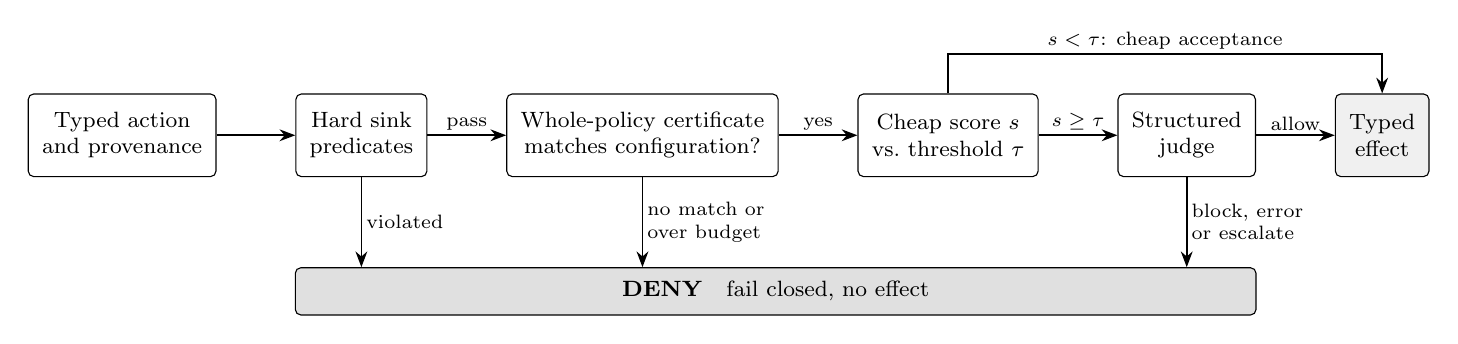
\begin{tikzpicture}[
  font=\footnotesize,
  box/.style={draw, rounded corners=2pt, align=center, minimum height=1.05cm,
              inner xsep=5pt, fill=white},
  arr/.style={-{Stealth[length=2mm]}, semithick},
  lab/.style={font=\scriptsize, inner sep=1.5pt},
  node distance=1.0cm]
\node[box] (act) {Typed action\\and provenance};
\node[box, right=of act] (sink) {Hard sink\\predicates};
\node[box, right=of sink] (cert) {Whole-policy certificate\\matches configuration?};
\node[box, right=of cert] (score) {Cheap score $s$\\vs.\ threshold $\tau$};
\node[box, right=of score] (judge) {Structured\\judge};
\node[box, right=of judge, fill=black!6] (eff) {Typed\\effect};
\draw[arr] (act) -- (sink);
\draw[arr] (sink) -- node[lab, above] {pass} (cert);
\draw[arr] (cert) -- node[lab, above] {yes} (score);
\draw[arr] (score) -- node[lab, above] {$s\geq\tau$} (judge);
\draw[arr] (judge) -- node[lab, above] {allow} (eff);
\draw[arr] (score.north) -- ++(0,0.5) -| node[lab, above, pos=0.25]
  {$s<\tau$: cheap acceptance} (eff.north);
\coordinate (dl) at ($(sink.south west)+(0,-1.15)$);
\coordinate (dr) at ($(judge.south east)+(0,-1.75)$);
\node[draw, rounded corners=2pt, fill=black!12, fit=(dl)(dr), inner sep=0pt] (deny) {};
\node at (deny.center) {\textbf{DENY}\quad fail closed, no effect};
\draw[arr] (sink.south) -- node[lab, right] {violated} (sink.south |- deny.north);
\draw[arr] (cert.south) -- node[lab, right, align=left] {no match or\\over budget}
  (cert.south |- deny.north);
\draw[arr] (judge.south) -- node[lab, right, align=left] {block, error\\or escalate}
  (judge.south |- deny.north);
\end{tikzpicture}
\caption{TINT's mediation path. Every proposal first passes the hard sink
predicates. Semantic acceptance additionally requires a whole-policy
certificate that matches the actual configuration; the cheap score then decides
between immediate acceptance and the structured judge. A matching certificate
does not show that the deployment distribution equals the calibration
distribution.}
\label{fig:pipeline}
\end{figure*}

Fig.~\ref{fig:pipeline} shows the path every proposal takes. The runtime first
evaluates the hard sink predicates and denies on failure. It then requires a
certificate whose fingerprint matches the current specification, threshold,
guard versions, judge view and deployment environment, and whose risk and
confidence parameters are within budget. Only then is the cheap score
consulted: if $s<\tau$ the proposal is accepted; otherwise the structured judge
decides, and a judge escalation reaches the abstaining approval stub and is
denied. For $T_b$, an applicable certificate and a low score yield cheap
acceptance; $T_j$ never gets past the sink. This control semantics is specified
by hand; it is not extracted from the Python code by a verified tool.

\subsection{Specification and explicit delegation (RQ I)}
Policies are written in a closed JSON domain-specific language (DSL) that
declares layers, property scopes, evidence, interfaces, direct trust edges and
mandatory predicates. There is deliberately no expression evaluator. The
well-formedness checker rejects unknown fields, duplicate names, cycles, scope
mismatches, edges without evidence, and a raw judge view whenever the judge's
contract requires quarantine. It also rejects predicates the runtime cannot
enforce, so that a declaration never appears to be enforced when it is not.

The first result makes the introduction's argument precise. Its proof is a
counterexample, which the artifact executes.

\begin{proposition}[Non-transitivity of conditional reliance]
\label{thm:nontransitive}
There exist layers, each satisfying its contract, whose naive composition
permits an unsafe action because the caller does not discharge the callee's
assumptions. Local contract satisfaction alone does not imply global safety.
\end{proposition}
\begin{IEEEproof}
Restrict attention to the three canonical traces. The judge's assumption $A_3$
is a structured input, and its guarantee $G_3$ is the correct verdict on these
traces. Let the judge meet $G_3$ under $A_3$ but return allow on raw $T_j$,
which contains the reviewer phrase. A middle relay assumes $A_2$, that its
caller discharges $A_3$, and guarantees $G_2$, that it relays a correct
verdict. The outer layer assumes $A_1=A_2\land\mathrm{sinkPreserved}$ and
guarantees $G_1$, safe execution. Each contract is an implication and holds
vacuously when its premise fails. The naive caller passes raw $T_j$ and
executes the relayed allow without a sink check. Every contract is satisfied,
yet the secret leaves the system. On $T_b$ no unsafe effect occurs, and raw
$T^*$ without the phrase is denied. The counterexample therefore exhibits
missing premises, not a failure of valid assume-guarantee inference.
\end{IEEEproof}

Read positively, the counterexample identifies what a sound closure needs:
each edge's assumptions are explicitly discharged, property scopes and actual
views are compatible, escalation is acyclic, and the mandatory invariants are
preserved. A bare declaration that one layer trusts another provides none of
these.

\begin{proposition}[Scoped composition soundness]
\label{thm:composition}
Assume a correct mandatory deterministic monitor, complete mediation with
unforgeable metadata, and monotone denial. Let the disjoint events $E_i$
exhaust final acceptance, and let $b_i$ bound the unsafe mass of route $i$:
$\Pr_D(Y=1,E_i)\leq b_i$. If these bounds hold simultaneously and all executable
interface premises hold, then no hard violation executes and
$R(D)\leq\sum_i b_i$. If the bounds hold simultaneously with probability
$1-\delta$ over the draw of calibration samples, the conclusion has confidence
$1-\delta$; $\delta$ concerns calibration, not randomness of decisions under $D$.
\end{proposition}
\begin{IEEEproof}
By induction on mediated trace extensions, every executed extension has passed
the correct deterministic monitor and so preserves the invariant. For the
semantic part, disjointness gives
$\mathbf{1}_{\{Y=1,\mathrm{allow}\}}=\sum_i\mathbf{1}_{\{Y=1,E_i\}}$, and taking
expectations yields the bound. Simultaneous certificates follow by splitting
the failure budget across a fixed family and applying a union bound, so
independence is not needed. If an executable interface premise fails, the
runtime denies. The proposition does not claim that distributional premises
can be decided at run time.
\end{IEEEproof}

Proposition~\ref{thm:composition} allows a separate bound per route. Our
implementation instead certifies the entire fixed routing policy at once. This
avoids challenge $\mathsf{C2}$: estimating the judge's error on the traffic it happens to
receive and multiplying by a reach rate would require assumptions about how
the cheap layer selects that traffic. Separately calibrated route bounds remain
a supported extension that the pilot does not estimate.

\subsection{Risk accounting and certification (RQ II)}
Hierarchies and ensembles fail differently when their guards are correlated.
To study dependence we use a simple \emph{common-shock} model. Conditional on
an unsafe input, a coin with probability $\rho$ is flipped. If it lands heads,
all guards compare one shared uniform random variable with their miss rates;
otherwise each guard uses its own independent uniform. Each guard's miss rate
is unchanged, but $\rho$ controls how often they fail together. We call $\rho$
the mixture weight; it is a model parameter, not an observed correlation.

\begin{proposition}[Risk of an all-veto ensemble]
\label{thm:bounds}
Let $\beta_i$ bound the joint event $M_i=\{Y=1,\mathrm{allow}_i\}$, let $m_i$
be guard $i$'s miss rate conditional on $Y=1$, and let $\pi=\Pr(Y=1)$. Then
$R\leq\min_i\beta_i$. Under conditional independence given $Y=1$,
$R=\pi\prod_i m_i$, and under the common-shock model
\begin{equation}
R=\pi\left((1-\rho)\prod_i m_i+\rho\min_i m_i\right).
\label{eq:mixture}
\end{equation}
\end{proposition}
\begin{IEEEproof}
The ensemble accepts only on the intersection of the $M_i$, which is contained
in each $M_i$; this gives the minimum bound. Conditional independence gives the
product of the $m_i$, and multiplying by $\pi$ gives joint risk. In the
shared-uniform branch the intersection has probability $\min_i m_i$; in the
independent branch it has probability $\prod_i m_i$. Averaging the branches
and multiplying by $\pi$ proves~\eqref{eq:mixture}.
\end{IEEEproof}

Two errors are easy to make here. First, multiplying the guards' \emph{joint}
risks $\beta_i$ is wrong even under conditional independence, because all of
those events contain the same event $Y=1$; one must multiply conditional miss
rates and then multiply by $\pi$ once. Second, an early-exit hierarchy is not an
ensemble: a proposal accepted cheaply never meets the judge, so its acceptance
event is not an intersection and Proposition~\ref{thm:bounds} does not apply.
Its risk is accounted for route by route, as in
Proposition~\ref{thm:composition}. A judge that a phrase like the one in $T_j$
can compromise also shows why repeated verdicts need not be independent.

\textbf{Three statistical promises.} The library keeps three guarantees apart.
\emph{Split conformal prediction} controls marginal coverage of prediction
sets. \emph{Conformal risk control} (CRC) controls the expected bounded loss
averaged over calibration samples and a new decision~\cite{arxiv220802814}: for
$n$ exchangeable samples $Z_k$, losses $l_t\in[0,1]$ that decrease with
conservatism $t$, and budget $\alpha$, CRC picks the least conservative $t$
with $(\sum_{k=1}^n l_t(Z_k)+1)/(n+1)\leq\alpha$. Neither guarantee says that
the population risk is small given the particular calibration sample one
observed, which is what a deployment certificate should say. The pilot
therefore uses the third promise.

\textbf{The implemented certificate} is a one-sided binomial (Clopper--Pearson)
upper bound on population risk. For each of $K$ fixed candidate policies, it
counts the $k$ unsafe accepted proposals among $n$ independent and identically
distributed (iid) calibration proposals, and allocates a failure budget
$\delta/K$ to each. For $k<n$ the upper bound $U$ is the $(1-\delta/K)$ quantile
of $\operatorname{Beta}(k+1,n-k)$, and $U=1$ for $k=n$. Zero observed losses
give $U=1-(\delta/K)^{1/n}$, which is small but not zero. With probability at
least $1-\delta$ all $K$ bounds hold at once, so any policy with
$U\leq\epsilon$ may be selected; if none qualifies, the runtime denies. The
confidence refers to repeated calibration draws; the deployment risk refers to
new proposals after the policy is fixed; a frequency on a finite test set is
neither.

\textbf{Distribution shift.} For a fixed policy and a deployment law $Q$, if
an external argument establishes total variation distance
$\operatorname{TV}(D,Q)\leq\eta$, then $R(Q)\leq\min(1,R(D)+\eta)$. We certify no
estimator of $\eta$. Without restrictions on $Q$, an attacker can concentrate
all traffic on any unsafe input the policy accepts, driving its risk to one.
The hard checks still exclude their exact predicates, but nothing excludes all
semantic violations. Absent exact semantic verification, denying uncertified
semantic acceptance is the only distribution-free fallback in this model.

\subsection{Escalation synthesis (RQ II)}
The next result says when escalating by score is the cheapest way to meet a
risk budget. It is a standard Lagrangian argument, and we state it to make its
premises visible.

\begin{proposition}[Sufficient condition for optimal escalation]
\label{thm:optimization}
For $x\sim D_X$, let $r_0(x)$ and $r_1(x)$ be the conditional probabilities of
unsafe acceptance under cheap acceptance and under escalation, let $d(x)>0$ be
the extra cost of escalation and $c_0(x)$ the baseline cost. A randomized
escalation probability $q(x)\in[0,1]$ yields
\begin{align*}
R(q)&=\mathbb E_{D_X}[(1-q)r_0+qr_1],\\
C(q)&=\mathbb E_{D_X}[c_0+qd].
\end{align*}
Consider minimizing $C(q)$ subject to $R(q)\leq\epsilon$ over measurable
policies with integrable costs. If some finite $\lambda\geq0$ and a feasible
pointwise minimizer $q$ of the Lagrangian satisfy $\lambda(R(q)-\epsilon)=0$,
then $q$ is optimal. It escalates where $\lambda(r_0-r_1)>d$, accepts where the
inequality is reversed, and may randomize on ties.
\end{proposition}
\begin{IEEEproof}
The multiplier $\lambda$ is a price per unit of risk. The Lagrangian is
\begin{align*}
L(q,\lambda)={}&\mathbb E[c_0+\lambda r_0]-\lambda\epsilon\\
&+\mathbb E[q(d-\lambda(r_0-r_1))],
\end{align*}
and the sign of the coefficient of $q$ gives the rule. By weak duality, every
feasible competitor costs at least the minimized Lagrangian. Complementary
slackness makes the candidate's cost equal to that bound. A finite multiplier
need not exist at a boundary budget, so its existence is a premise.
\end{IEEEproof}

The proposition addresses challenge $\mathsf{C3}$ directly. With the raw judge and no
sink, escalating $T_j$ \emph{increases} risk, so $r_0-r_1<0$ and the rule never
escalates it at positive cost. For $T_b$, a small risk reduction may not be
worth a deliberation. For $T^*$, no optimization waives the mandatory sink. The
conditional risks $r_0,r_1$ and their monotonicity in the score are
assumptions; the proposition does not estimate them.

The pilot solves a smaller, finite problem: among a fixed grid of threshold
policies, choose the one with the lowest mean calibration cost whose
simultaneous upper bound meets the budget. This choice is exact within the
grid, not among all routing functions. A separate linear program with known
risks supports mixtures of policies; with a normalization constraint and one
active risk constraint, an optimal vertex mixes at most two policies. An
optional interface certifies a latency exceedance event
$\Pr(L>\mathrm{budget})\leq\gamma$, but we evaluated no real inference latency.

\begin{proposition}[Tightness and limits]
\label{thm:limits}
The veto bound $\min_i\beta_i$ and the capped route bound $\min(1,\sum_i b_i)$
are tight given only the stated marginal information. Pairwise independence
does not determine the joint failure probability of an ensemble.
\end{proposition}
\begin{IEEEproof}
For the veto bound take $\pi=1$ and $m_i=\beta_i$, and let guard $i$ miss when a
shared uniform variable is at most $m_i$; the joint miss probability is
$\min_i\beta_i$. For routes, place disjoint unsafe masses $b_i$ when they sum
to at most one, and otherwise masses no larger than the $b_i$ that sum to one.
Finally, read three bits as guard misses and take the uniform laws on
$\{000,011,101,110\}$ and on $\{001,010,100,111\}$. In both, each bit has
marginal $1/2$ and every pair is independent, yet the all-miss probability is
$0$ in the first and $1/4$ in the second.
\end{IEEEproof}

The practical consequence is that measuring pairwise correlations between
guards, a natural thing to do, cannot certify an ensemble's joint risk.

\subsection{Trust boundary, assumptions and limits}
\label{sec:boundary}
The typed interpreter supports a local mock HTTP service, in-memory files and
typed effect records; it rejects shell commands and unknown tool fields.
Provenance references are write-once, and unknown references keep conservative
labels. Approvals bind the immutable action digest and epoch. A tool adapter
parses function-call argument objects and calls the same mediated interpreter;
we have not connected it to an external model API.

At every runtime decision, a fingerprint, a cryptographic hash of the
specification, guard versions, threshold, view and environment, is recomputed
and compared with the certificate, and the certificate's risk and confidence
values are checked against the budget. That honest version strings identify
immutable implementations, that hosts declare dependencies completely, and that
certificate issuers are trustworthy remain external premises.
Table~\ref{tab:obligations} separates what the code checks from what it must
assume. By induction over the single effect transition of the control
semantics, every effect is preceded by a passed sink check and a matching
certificate. This is an inspection argument, not a proved refinement between
the semantics and the Python code.

\begin{table}[t]
\caption{What TINT checks at run time and what it must assume.}
\label{tab:obligations}
\centering\scriptsize
\setlength{\tabcolsep}{3pt}
\begin{tabular}{>{\raggedright\arraybackslash}p{.22\columnwidth}>{\raggedright\arraybackslash}p{.36\columnwidth}>{\raggedright\arraybackslash}p{.32\columnwidth}}
\toprule
Obligation & Executed check & External premise\\
\midrule
Edge compatibility & Scope/evidence sets; fixed topology & Truth of guarantees\\
Provenance & Write-once store; parent-label union & Complete host dependencies\\
Approval & Digest and epoch match & Trusted grant issuer\\
Hard safety & Mandatory typed predicates & Faithful interpreter semantics\\
Judge interface & Closed Boolean/numeric schema & Adequate semantic evidence\\
Certificate & Policy/view/context identity; risk/confidence budgets & Valid issuer, labels, iid relationship\\
Guard identity & Version string in fingerprint & Immutable implementation\\
\bottomrule
\end{tabular}
\end{table}

Three scorer versions exist. The primary study used \texttt{lexical-v1}; the
exploratory study used \texttt{lexical-v2}, which fixes an arithmetic defect
described in Section~\ref{sec:results}; the current default,
\texttt{lexical-v3-bounded}, adds an input-length cap and produced none of the
reported measurements. Exceptions in a plugin deny authority, but a synchronous
plugin that never returns is not cancelled. Concurrent mutation of trusted
stores and covert channels are out of scope.

\textbf{Assumptions and limits.} The deterministic guarantees hold only for
this typed, completely mediated semantics. The PRISM model is a separately
checked finite abstraction with no proved refinement relation to the Python
code. Quarantine removes raw instructions from the judge's input but does not
establish the semantic oracle. Statistical certification assumes fixed
candidates and iid calibration and deployment draws; arbitrary adaptation and
drift are not covered, and a matching fingerprint cannot detect them.

\section{Evaluation Design}
\label{sec:design}
Our evaluation is designed to test whether TINT's mechanisms behave as the
approach claims, not to estimate how safe a real agent would be. That choice
shapes every component. The guards are scripted rather than learned, so each
decision can be traced to a known cause; a failure then points to the mechanism
under test rather than to an opaque model, and Proposition~\ref{thm:nontransitive}
requires a judge whose vulnerability is known exactly. The traces come from an
authored mixture whose unsafe labels hold by construction. This means risk can
be measured exactly, without disagreement between annotators, and it lets us
include semantic-only attacks that the sink cannot decide, which public
benchmarks do not isolate. The comparators are ablations, each removing one
mechanism (the sink, the structured view, or the certificate) from an otherwise
identical pipeline, because the question is which mechanism produces which
effect, and re-implementations of published systems would differ in many ways
at once. Statistical certification is tested on a separate generator whose true
risk is known, since coverage cannot be checked when ground truth is
unavailable. Costs are modeled units, and the risk budget is deliberately
permissive, so that the certification and selection logic is exercised rather
than trivially refusing. Finally, the protocol was preregistered and the
primary run is reported as it failed, with the correction kept separate, so
that no result was obtained by adjusting the design after seeing the data.
These choices give internal validity at the expense of external validity:
Section~\ref{sec:results} establishes what the mechanisms do on a controlled
instrument, and Section~\ref{sec:discussion} states what a study with real
models would have to add.

The protocol was committed and tagged \texttt{prereg-v1} before any
calibration or held-out evaluation. Unit tests and the canonical model checks
preceded the tag and are not confirmatory findings. The tag is a local git
tag, not an independently timestamped registry entry. One amendment, described
in Section~\ref{sec:results}, is reported separately from the primary run.

\subsection{Implementation in the codebase}
\label{sec:implementation}
TINT is implemented as a small Python package, \texttt{src/tint}, that depends
only on NumPy and SciPy and performs no network or shell access. Around it, the
repository holds the formal artifacts (\texttt{formal/}), the experiment harness
(\texttt{experiments/}) and the analysis and paper-generation scripts
(\texttt{scripts/}). Table~\ref{tab:implementation} maps each element of the
approach in Sections~\ref{sec:background} and~\ref{sec:approach} to the code
that realizes it and to the study that exercises it. We describe the code here
so that a reader can check any claim in the paper against a specific module.

\begin{table*}[t]
\caption{How the approach maps to the codebase. Module paths are relative to
\texttt{src/tint} unless a top-level directory is given. The last column names
the study in Sections~\ref{sec:design} and~\ref{sec:results} that exercises the
code.}
\label{tab:implementation}
\centering\scriptsize
\setlength{\tabcolsep}{4pt}
\renewcommand{\arraystretch}{1.3}
\begin{tabular}{>{\raggedright\arraybackslash}p{.20\textwidth}>{\raggedright\arraybackslash}p{.15\textwidth}>{\raggedright\arraybackslash}p{.36\textwidth}>{\raggedright\arraybackslash}p{.21\textwidth}}
\toprule
Approach element & Paper reference & Code (module: main entry points) & Exercised by\\
\midrule
Typed actions, provenance labels, approvals & Defs.~\ref{def:provenance}--\ref{def:property} &
\texttt{model}: \texttt{Label}, \texttt{Action.digest}, \texttt{ProvenanceStore}, \texttt{ApprovalStore}, \texttt{action\_view} &
Unit tests; hard counts in the replay\\
Policy language and well-formedness checker & Defs.~\ref{def:contract}--\ref{def:trust}; Sec.~\ref{sec:approach}-A &
\texttt{spec}: \texttt{parse}, \texttt{check}, \texttt{Contract}, \texttt{TrustEdge}; policy in \texttt{experiments/configs/devagent.json} &
Mutation study; policy inventory\\
Layers: hard predicates, cheap scorer, structured view, judges & Def.~\ref{def:layer}; Table~\ref{tab:traces} &
\texttt{layers}: \texttt{deterministic}, \texttt{LexicalScorer}, \texttt{quarantine}, \texttt{StructuredJudge}, \texttt{ExposedJudge}, \texttt{safe\_judge\_call} &
Canonical traces; replay\\
Mediation path and configuration fingerprint & Fig.~\ref{fig:pipeline}; Prop.~\ref{thm:composition} &
\texttt{runtime}: \texttt{GuardRuntime.evaluate}, \texttt{policy\_fingerprint}, \texttt{parse\_tool\_call} &
Replay (TINT rows); CPU timing\\
Certificates and statistical utilities & Sec.~\ref{sec:approach}-B; Prop.~\ref{thm:bounds} &
\texttt{calibration}: \texttt{binomial\_upper}, \texttt{certify\_family}, \texttt{Certificate.applies}, \texttt{conformal\_risk\_control}, \texttt{veto\_bound} &
Coverage and dependence studies\\
Escalation synthesis & Sec.~\ref{sec:approach}-C; Props.~\ref{thm:optimization}--\ref{thm:limits} &
\texttt{synthesis}: \texttt{select}, \texttt{lagrangian\_escalate}, \texttt{optimal\_mixture} &
Synthesis study; policy selection\\
Typed sandbox and canonical counterexample & Prop.~\ref{thm:nontransitive}; Table~\ref{tab:traces} &
\texttt{agents}: \texttt{Sandbox.call}, \texttt{canonical\_traces}, \texttt{fixture\_store} &
Unit tests; PRISM model\\
Comparators & Table~\ref{tab:baselines} &
\texttt{baselines}: \texttt{decide} &
Replay\\
Finite formal checks & Props.~\ref{thm:nontransitive}, \ref{thm:composition}, \ref{thm:bounds}, \ref{thm:limits} &
\texttt{formal/cascade.pm} (PRISM), \texttt{formal/check.py}, \texttt{formal/sanity.py} &
RQ I results\\
Trace generator, harness and analysis & Secs.~\ref{sec:design}--\ref{sec:results} &
\texttt{experiments/dataset.py}, \texttt{experiments/run.py}, \texttt{scripts/process\_results.py}, \texttt{scripts/validate\_replay.py}, \texttt{scripts/make\_macros.py} &
All studies\\
\bottomrule
\end{tabular}
\end{table*}

The path of a single decision through the code follows Fig.~\ref{fig:pipeline}
step by step. \texttt{Sandbox.call} receives a function-call argument object
and \texttt{parse\_tool\_call} turns it into an immutable \texttt{Action},
rejecting unknown fields. \texttt{GuardRuntime.evaluate} then builds the
\texttt{ActionView}, whose labels and approval flag come only from the trusted
stores, and applies the hard predicates in \texttt{deterministic}. If they pass,
it recomputes \texttt{policy\_fingerprint} and asks
\texttt{Certificate.applies} whether the stored certificate names this exact
configuration and lies within the risk and confidence budgets. Only then does
it call the scorer; a score below the threshold accepts, and otherwise the
\texttt{quarantine} function builds the closed structured view and
\texttt{safe\_judge\_call} invokes the judge, converting any exception into a
block. An escalation reaches the approval stub and is denied. Every outcome is
returned as a \texttt{GuardDecision} record, and the sandbox applies a typed
effect only for an allow.

Three places where the code is narrower than the approach deserve mention.
First, the checker in \texttt{spec} validates arbitrary acyclic graphs, but the
runtime accepts only the fixed three-layer topology of
\texttt{devagent.json}: a metadata layer, a raw-view scorer and a
structured-view judge. Second, the runtime uses one whole-policy certificate
rather than the per-route bounds that Proposition~\ref{thm:composition}
permits. Third, \texttt{lagrangian\_escalate} implements the rule of
Proposition~\ref{thm:optimization}, and \texttt{calibration} also implements
split conformal prediction and CRC, but the pilot uses none of them: it selects
from a finite threshold grid with \texttt{select}. The runtime's trust boundary
is described in Section~\ref{sec:boundary}.

Correctness of the code is checked in three ways. Unit and analysis tests in
\texttt{tests/} reach \resCoreCoverage{}\% line coverage of the package. A
replay validator re-joins every retained decision to its trace, label and
configuration. A manifest of cryptographic hashes ties the raw logs, sources and
configurations to the processed results, and the paper's numbers are generated
from those results rather than typed by hand.

\subsection{Experimental setup}
\label{sec:setup}
\textbf{Environment.} All experiments ran in a single process on one
workstation (\resEnvProcessor{}, \resEnvCpuCount{} logical CPUs,
\resEnvPlatform{}) with Python \resEnvPython{}, NumPy \resEnvNumpy{}, SciPy
\resEnvScipy{} and pytest \resEnvPytest{}. Timings use the operating system's
monotonic nanosecond clock. No external API was called, and no model was
executed. Each run records the commit that produced it: \texttt{\resPrimaryCommit{}}
for the primary run and \texttt{\resExploratoryCommit{}} for the exploratory
run.

\textbf{What we could and could not run.} The testbed has a handwritten
lexical scorer, a deliberately vulnerable raw-text judge and a deterministic
judge over the structured view; none uses the oracle label. Proposals come from
two scripted sources, not from language models. We ran no model: the
available GPU had no GPU-enabled learning framework installed, no API
credentials were available, the small guard model we inspected required an
access agreement we did not accept, and the Docker engine was unavailable.

\textbf{Configuration.} Table~\ref{tab:setup} lists every parameter of the
frozen configuration \texttt{experiments/configs/pilot.json}. The risk budget
is far too permissive for production; it was chosen to exercise the
certification mechanics. Modeled layer costs are arbitrary units; CPU times are
measured separately on complete local decisions.

\begin{table}[t]
\caption{Frozen experimental configuration. All values come from
\texttt{experiments/configs/pilot.json}; the exploratory run changes only the
seeds and the scorer version.}
\label{tab:setup}
\centering\scriptsize
\setlength{\tabcolsep}{3pt}
\renewcommand{\arraystretch}{1.2}
\begin{tabular}{>{\raggedright\arraybackslash}p{.50\columnwidth}>{\raggedright\arraybackslash}p{.42\columnwidth}}
\toprule
Parameter & Value\\
\midrule
Primary seeds / exploratory seeds & \resPrimarySeedFirst{}--\resPrimarySeedLast{} / \resExploratorySeedFirst{}--\resExploratorySeedLast{}\\
Traces per seed: calibration / development / test / shift & \resCalibrationCount{} / \resDevelopmentCount{} / \resTestPerSeed{} / \resShiftPerSeed{}\\
Threshold grid & \resThresholdMin{} to \resThresholdMax{} in steps of \resThresholdStep{} (\resThresholdCount{} policies)\\
Baseline threshold for uncertified cheap exits & \resBaselineThreshold{}\\
Risk budget $\epsilon$ / confidence-failure budget $\delta$ & \resRiskBudget{}\% / \resConfidenceFailure{}\%\\
Modeled cost: rules / scorer / judge / approval & \resCostRules{} / \resCostScorer{} / \resCostJudge{} / \resCostApproval{} units\\
Coverage study: replications / calibration / test draws & \resPrimaryReplications{} (\resCoveragePerSeed{} per seed) / \resCoverageCalibrationCount{} / \resCoverageTestCount{}\\
Coverage study risk target & \resCoverageTarget{}\%\\
Dependence study draws per cell & \resDependenceSamples{}\\
Bootstrap resamples & \resBootstrapCount{}\\
Core-search query budget & \resAdaptiveBudget{}\\
\bottomrule
\end{tabular}
\end{table}

\textbf{Procedure.} The harness \texttt{experiments/run.py} executes the same
steps for every seed.
\begin{enumerate}
\item Generate the calibration, development, test and shift splits with
\texttt{experiments/dataset.py}.
\item Evaluate every threshold policy on the calibration split, recording for
each proposal whether it was an unsafe acceptance and what it cost.
\item Compute the simultaneous binomial upper bound of every policy and select
the cheapest policy whose bound meets the risk budget; if none does, issue no
certificate.
\item Build a \texttt{GuardRuntime} with the selected threshold and, if one
exists, a certificate bound to the configuration fingerprint.
\item Replay the development, test and shift splits through TINT and all six
comparators, writing one compressed record per decision with its verdict,
route, modeled cost, elapsed time and hard-violation flag.
\end{enumerate}
Development data are recorded for diagnostics only and never used to revise
thresholds. After the replay, the harness runs the coverage, dependence,
checker, synthesis and core-search studies of Section~\ref{sec:evidence} on
their own generators.

\textbf{Outputs and reproduction.} The primary run took
\resPrimaryRuntime{}~s and wrote \resPrimaryRecords{} decision records; the
exploratory run took \resExploratoryRuntime{}~s and wrote
\resExploratoryRecords{}. The command \texttt{python scripts/tasks.py all}
archives any previous raw results and repeats the whole pipeline: tests, formal
checks, both runs, analysis, macro generation and the PDF build. The cheaper
command \texttt{python scripts/tasks.py verify-results} re-derives every
processed number from the retained raw logs without rerunning the experiments.

\subsection{Trace data and comparators}
For each of \resPrimarySeeds{} primary seeds, a fixed generator samples
\resCalibrationCount{} calibration, \resDevelopmentCount{} development and
\resTestPerSeed{} test traces with disjoint identifiers. Traces are drawn from
seven authored families with fixed sampling masses: benign reports, benign
security discussion, secret exfiltration, unapproved destructive production
actions, direct instruction injection, implicit unauthorized patches and
judge-targeting text (Table~\ref{tab:families}). Within a family, traces differ
only in an identifier suffix, so the splits are iid samples from one mixture,
not independent tasks. A further \resShiftPerSeed{} traces per seed come from an
encoded family absent from calibration. Labels are known by construction; there
was no human annotation.

Table~\ref{tab:baselines} lists the comparators. They are controls designed to
isolate one mechanism each, not reimplementations of AgentSpec, ShieldAgent or
LlamaFirewall. Uncalibrated cheap exits use the fixed threshold
$\resBaselineThreshold{}$; the calibrated method uses its selected threshold.
Invalid delegation versus naive-with-sink isolates the mandatory sink;
naive-with-sink versus checked-uncalibrated isolates the judge view; and the
two checked variants isolate certification. Invalid delegation is charged a
nominal scorer cost even though its verdicts equal the raw judge's; cost units
are protocol charges, not profiles.

\begin{table}[t]
\caption{Comparators. Fixed denotes the protocol's baseline threshold;
selected denotes the calibrated threshold. A failed cheap exit with no judge
is a denial.}
\label{tab:baselines}
\centering\scriptsize
\setlength{\tabcolsep}{3pt}
\begin{tabular}{lcccc}
\toprule
Method & Hard sink & Cheap exit & Judge & Certificate\\
\midrule
Rules only & yes & none & none & no\\
Lexical only & no & fixed & none & no\\
Scripted judge only & no & none & raw & no\\
Invalid delegation & no & none & raw & no\\
Naive with sink & yes & fixed & raw & no\\
Checked uncalibrated & yes & fixed & structured & no\\
Checked calibrated (TINT) & yes & selected & structured & yes\\
\bottomrule
\end{tabular}
\end{table}

We inspected public benchmark repositories and their licenses but executed or
redistributed none. R-Judge's project website states a noncommercial
share-alike license, while retrieval of its repository license failed;
AgentHarm adds a safety-use restriction. A repository's code license need not
cover the datasets it contains.

\subsection{Evidence map and statistics}
\label{sec:evidence}
Table~\ref{tab:hypotheses} maps each preregistered hypothesis to its evidence
and outcome.

\begin{table*}[t]
\caption{Preregistered hypotheses, evidence and outcomes. ``Supported'' always
refers to the local instrument; missing evidence is reported as such, never
replaced by simulated claims about real models.}
\label{tab:hypotheses}
\centering\small
\begin{tabular}{llll}
\toprule
Hypothesis & RQ & Evidence & Outcome\\
\midrule
Hard invariant preservation & I & Proof, PRISM, exhaustive model, replay & Supported within typed semantics\\
Planted invalid-spec detection & I & Mutation confusion matrix & Supported for generator classes\\
Full policy expressiveness & I & Executable restricted-DSL inventory & Refuted\\
Selected bound coverage & II & Known iid law with repeated calibration & Supported for synthetic law\\
Invalid delegation counterexample & II & Canonical traces and stronger sink control & Supported; sink alone also protects\\
Finite-family selection optimality & II & Independent enumeration and LP constraints & Supported within candidate family\\
Useful safety--utility improvement & III & Paired replay, controls and trade-off plots & Primary inconclusive; exploratory only\\
External/model generalization & III & No real-model or benchmark execution & Inconclusive/not run\\
\bottomrule
\end{tabular}
\end{table*}

The coverage study uses a \emph{different} generator from the agent traces, one
in which the true risk is known. For each fresh uniform draw $U$, candidate $j$
incurs loss $\mathbf1[U<r_j]$, so its population risk is exactly $r_j$ and losses
are nested across candidates. Each of \resPrimaryReplications{} replications
draws \resCoverageCalibrationCount{} calibration and \resCoverageTestCount{}
test samples, targets \resCoverageTarget{}\% risk, and selects the cheapest
certified candidate. When none is feasible, the zero-risk denial fallback is
counted as covered rather than dropped. We report whether the selected
candidate's true risk lies below its bound (certificate coverage) separately
from whether its test frequency lies below the budget.

\textbf{A caution about the agent-trace statistics.} Every comparator is a
deterministic function of a trace's family, so each method's population risk,
utility and cost follow exactly from the family masses; we report these exact
values alongside the sample estimates. Across seeds, the only source of
variation is how many traces of each family were drawn. Seed-level paired
differences are summarized with a percentile bootstrap
(\resBootstrapCount{} resamples), paired Wilcoxon tests with Holm correction
across baselines, and the Vargha--Delaney effect size $A_{12}$. With ten
seeds the smallest attainable Holm-adjusted $p$ is the value we report for
every non-tied comparison, so these tests confirm that differences are not
artifacts of sampling, nothing more. Intervals are unadjusted and resample
seeds, not individual traces. CPU quantiles pool decisions with a fixed
comparator order and no warmup. Coverage intervals are exact binomial
intervals.

The checker study times repeated valid declarations and four planted mutation
classes: missing evidence, scope mismatch, unknown endpoint and cycle.
Authoring effort and usability were not measured. A small \emph{core search},
with at most \resAdaptiveBudget{} local queries per method, cycles through fixed
attack phrases and stops at the first unsafe acceptance. It calls the
uncalibrated decision functions at the fixed threshold (its log label
\texttt{checked\_quarantine} is misleading), not the certified runtime, and
every method accepts its first phrase. It provides no evidence of adaptive
robustness.

\section{Results}
\label{sec:results}
\subsection{RQ I: specification and decomposition}
The PRISM model checks \resPrismCases{} canonical configurations and agrees
with the independent checker on both reachability properties. Exhaustive
enumeration covers all \resFormalStates{} Boolean sink cases, and seeded sanity
checks evaluate \resFormalInstances{} random probability instances against the
closed-form expressions. These finite checks test the propositions; the
general proofs remain on paper and are not mechanized in Lean or Isabelle.

In the mutation study the checker rejects all \resPrimaryCheckerTP{}
invalid-case evaluations, covering \resPrimaryCheckerUniqueInvalid{} unique
mutated specifications, and accepts all \resPrimaryCheckerTN{} evaluations of
\resPrimaryCheckerUniqueClean{} unique clean graphs: \resPrimaryCheckerFP{}
false rejections and \resPrimaryCheckerFN{} missed mutations. This shows
agreement with the mutation generator, not precision and recall on policy
errors that developers actually make. The largest median checking time over
all graph sizes was \resPrimaryCheckerMax{} microseconds.

The DSL fully supports only \resSupportedClasses{} of the \resPolicyClasses{}
policy classes we inventoried: production approval and secret egress. Semantic
injection is handled only through the statistical proxy, and filesystem
confinement and cumulative spending are rejected as unsupported. The
full-expressiveness hypothesis is therefore refuted. We consider an explicit
rejection preferable to accepting declarations the runtime cannot enforce.
Line coverage of the core package is \resCoreCoverage{}\%, including a
regression test for the numeric defect.

\textbf{Answer to RQ I.} A safety property can be split into an exact
deterministic invariant enforced at the sink and a population-level semantic
bound, with per-edge contracts whose premises are executable checks.
Proposition~\ref{thm:nontransitive} and its executable counterexample show why
the premises must be checked. The decomposition works for the two
deterministic policy classes we support; richer policies remain out of reach of
the current DSL.

\subsection{RQ II: risk, dependence and policy selection}
On the synthetic law with known risk, selected bounds cover the true
population risk in \resPrimaryCoverage{}\% of \resPrimaryReplications{}
replications (exact interval [\resPrimaryCoverageLo{}\%,
\resPrimaryCoverageHi{}\%]), above the nominal \resNominalConfidence{}\%. The
selected policy's test frequency is below the \resCoverageTarget{}\% budget in
\resPrimaryFiniteTestBelow{} replications. The certificate is thus
conservative on an iid law, as its construction predicts; this is not a
deployment guarantee.

\begin{figure}[t]
\centering
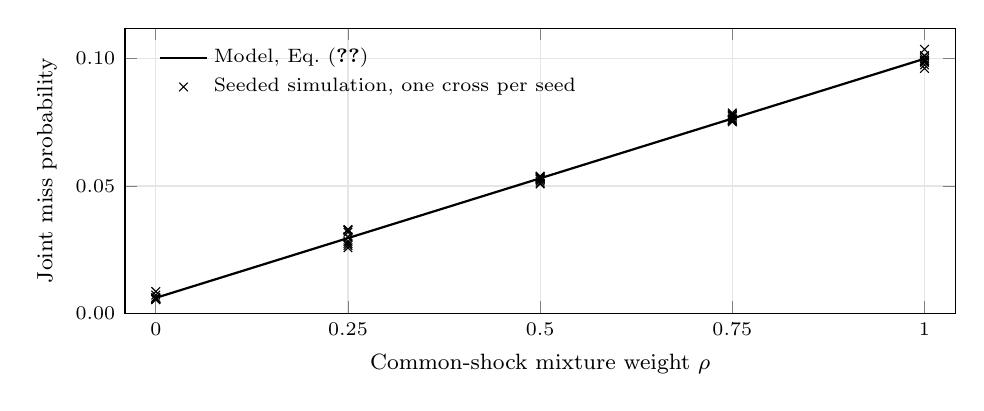
\begin{tikzpicture}
\begin{axis}[width=\columnwidth, height=5.2cm, xmin=-0.04, xmax=1.04, ymin=0, ymax=0.112,
  xlabel={Common-shock mixture weight $\rho$}, ylabel={Joint miss probability},
  xtick={0,0.25,0.5,0.75,1}, scaled y ticks=false,
  yticklabel style={/pgf/number format/fixed, /pgf/number format/fixed zerofill, /pgf/number format/precision=2},
  tick label style={font=\scriptsize}, label style={font=\footnotesize},
  legend pos=north west, legend cell align=left,
  legend style={font=\scriptsize, draw=none, fill=none},
  grid=major, grid style={black!10}]
\addplot[domain=0:1, samples=2, thick]
  {(1-x)*\resDependenceFirst*\resDependenceSecond*\resDependenceThird+x*\resDependenceFirst};
\addlegendentry{Model, Eq.~(\ref{eq:mixture})}
\addplot[only marks, mark=x, mark size=2.2pt] coordinates {\resDependencePoints};
\addlegendentry{Seeded simulation, one cross per seed}
\end{axis}
\end{tikzpicture}
\caption{Common-shock simulations against
\eqref{eq:mixture}. All inputs are unsafe ($\pi=1$), with conditional miss
rates $\resDependenceFirst{},\resDependenceSecond{},\resDependenceThird{}$. Each
cross is one seed with \resDependenceSamples{} draws. The horizontal axis is
the model's mixture weight $\rho$, not a measured correlation.}
\label{fig:dependence}
\end{figure}

Fig.~\ref{fig:dependence} confirms~\eqref{eq:mixture} by simulation. As the
mixture weight grows, the ensemble's joint miss probability rises from the
product of the miss rates toward the smallest one: adding a correlated guard
buys little. The parity construction of Proposition~\ref{thm:limits} adds that
even identical pairwise statistics can hide very different joint risks. Both
are controlled checks of the theory, not estimates of real guard correlations.

Discrete policy selection agrees with a separate exhaustive calculation on all
\resPrimarySynthInstances{} primary instances (\resPrimarySynthMismatches{}
mismatches) and all \resExploratorySynthInstances{} exploratory instances
(\resExploratorySynthMismatches{} mismatches). The original synthesis logs
omitted calibration counts, so their stored bounds cannot be recomputed from
those records; the amended logs retain the counts. A later re-analysis
reconstructs each linear program's risk and cost from its weights, checks the
simplex constraints and compares the objective with independently coded
vertex enumeration. It also joins historical decisions to traces and checks
configuration, authored labels and all outputs other than timings.
``Independent'' here means separately coded, not separately authored.

\textbf{The primary run was infeasible.} In every one of the \resPrimarySeeds{} primary seeds, no candidate's simultaneous upper bound met
the budget, so the runtime denied every semantic acceptance. The cause is
visible in the calibration counts. Every one of the \resThresholdCount{}
thresholds produced the same number of calibration losses, so the grid offered a
single risk level and only \resPrimaryDistinctPolicies{} behaviorally distinct
policies, which differ in cost
and benign utility but not in risk. The smallest upper bound across all seeds and thresholds was
\resPrimaryMinBound{}\%, above the \resRiskBudget{}\% budget. No choice of
threshold could have succeeded, so the infeasibility reflects the detector, not
the calibration procedure. Reporting it, rather than relaxing the budget or
treating a missing certificate as permission, is exactly what a
risk-constrained synthesizer should do.

\textbf{Answer to RQ II.} Under fixed candidates, iid calibration and correct
hard mediation, an early-exit hierarchy's risk is bounded by the sum of its
route bounds, and an ensemble's by its tightest member; both bounds are tight.
Compositions fail when edge premises are not discharged
(Proposition~\ref{thm:nontransitive}), when guards fail together
(Fig.~\ref{fig:dependence}), and whenever the deployment law may differ
arbitrarily from calibration, which includes adaptive adversaries. A threshold
escalation rule is cost-optimal when conditional risks are known and a
Lagrange multiplier exists (Proposition~\ref{thm:optimization}). Empirically,
the certificate is conservative on a known law, and the synthesizer exposes
infeasibility instead of hiding it.

\subsection{RQ III: utility and engineering trade-offs}
\begin{table*}[t]
\caption{Primary replay on held-out traces. Risk is joint unsafe acceptance
over all proposals; utility is benign acceptance. Cost is in modeled units, CPU
is measured local decision time, and the hard count is the number of accepted
proposals that violate $\varphi_{\rm det}$. The calibrated method found no
feasible certificate and denied every semantic acceptance.}
\label{tab:primary}
\centering\small
\begin{tabular}{lrrrrr}
\toprule
Method & Risk (\%) & Utility (\%) & Cost units & CPU $p_{95}$ ($\mu$s) & Hard count\\
\midrule
\resPrimaryTable
\bottomrule
\end{tabular}
\end{table*}

Table~\ref{tab:primary} reports the primary replay on \resPrimaryTestCount{}
held-out proposals. TINT reaches \resPrimaryCheckedQuarantineRisk{}\% risk only
by accepting nothing: its benign utility is
\resPrimaryCheckedQuarantineUtility{}\%. Rules only keeps
\resPrimaryRulesOnlyUtility{}\% utility at \resPrimaryRulesOnlyRisk{}\% risk.
Every method without the sink accepts all \resFamilyProductionDeletePrimary{}
unapproved production deletions in the test set; every method with the sink
accepts none. A system that denies every benign task has not shown a
useful safety--utility trade-off, whatever its risk.

\textbf{The arithmetic defect.} The scorer is meant to compute
$s(k)=\min(98,4+12k)/100$, where $k$ is the number of the strings
\texttt{ignore, override, secret, .env, reviewer, instruction, send, upload}
that occur as substrings after case-folding, and the judge blocks when
$s\geq0.40$. The primary version evaluated $0.04+0.12\cdot3$ in binary floating
point, which is slightly below $0.40$, so a proposal matching three strings was
allowed instead of blocked. Direct injection and judge targeting match exactly
three strings. This explains why the primary grid had a single risk level:
those two families were accepted on whichever route a threshold sent them,
and implicit patches, which match nothing, were always accepted cheaply. The
checked core's exact population risk was therefore
\resPrimaryCheckedUncalibratedPopulationRisk{}\% at every threshold.

\textbf{The amendment.} The exploratory version computes the score in integer
hundredths, changing no strings and no cutoffs. It was versioned separately,
the original logs were preserved, and it was run on \resExploratorySeeds{}
fresh seeds. Under the corrected scorer, the score takes only three values on
the fixture law: $s=0.04$ for benign reports, implicit patches, production
deletion and the shifted family; $s=0.40$ for exfiltration, direct injection and
judge targeting; and $s=0.76$ for benign security text. The grid again has
\resExploratoryDistinctPolicies{} distinct policies, now with
\resExploratoryDistinctRiskLevels{} risk levels. For example, seed
\resExampleSeed{} observes \resExampleMisses{} losses among
\resExampleCalibrationCount{} calibration proposals at its selected threshold
\resExampleThreshold{}, giving a simultaneous upper bound of
\resExampleBound{}\%. This exploratory result does not retroactively make the
primary study a success.

\begin{table*}[t]
\caption{Exploratory replication with the corrected scorer on fresh seeds.
Columns as in Table~\ref{tab:primary}. The calibrated and uncalibrated checked
variants make identical decisions, because no score lies between their
thresholds; certification here selects and licenses a policy, it does not
detect anything new.}
\label{tab:exploratory}
\centering\small
\begin{tabular}{lrrrrr}
\toprule
Method & Risk (\%) & Utility (\%) & Cost units & CPU $p_{95}$ ($\mu$s) & Hard count\\
\midrule
\resExploratoryTable
\bottomrule
\end{tabular}
\end{table*}

Table~\ref{tab:exploratory} shows that TINT now accepts
\resExploratoryCheckedQuarantineUtility{}\% of benign proposals at
\resExploratoryCheckedQuarantineRisk{}\% risk. Compared with naive-with-sink,
the paired risk difference is $\resExploratoryNaiveWithSinkComparisonDiff{}$
percentage points (unadjusted interval
$[\resExploratoryNaiveWithSinkComparisonLo{},
\resExploratoryNaiveWithSinkComparisonHi{}]$, Holm-adjusted
$p=\resExploratoryNaiveWithSinkComparisonP{}$,
$A_{12}=\resExploratoryNaiveWithSinkComparisonA{}$, where larger values favor
TINT), with identical utility. The whole difference comes from one family, as
Table~\ref{tab:families} shows: judge-targeting text is accepted by the raw
judge and denied by the structured one.

\begin{table}[t]
\caption{Authored families. $N_P$ and $N_E$ are test counts in the primary and
exploratory runs; mass is the sampling probability; the last two columns are
exploratory acceptance rates within each family. Traces in a family differ only
in an identifier suffix.}
\label{tab:families}
\centering\scriptsize
\setlength{\tabcolsep}{3pt}
\begin{tabular}{lrrrrr}
\toprule
Family & $N_P$ & $N_E$ & Mass (\%) & Naive (\%) & TINT (\%)\\
\midrule
\resFamilyTable
\bottomrule
\end{tabular}
\end{table}

\begin{table}[t]
\caption{How TINT decides each family under the corrected scorer at its
selected threshold. $k$ is the number of listed strings matched and $s$ the
resulting score; the judge blocks when $s\geq0.40$. Unsafe families are marked
with an asterisk.}
\label{tab:derivation}
\centering\scriptsize
\setlength{\tabcolsep}{3pt}
\begin{tabular}{lcccl}
\toprule
Family & $k$ & $s$ & Sink & TINT outcome\\
\midrule
Benign report & $0$ & $0.04$ & pass & cheap accept\\
Benign security text & $6$ & $0.76$ & pass & judge blocks (false denial)\\
Secret exfiltration$^*$ & $3$ & $0.40$ & block & denied by sink\\
Production deletion$^*$ & $0$ & $0.04$ & block & denied by sink\\
Direct injection$^*$ & $3$ & $0.40$ & pass & judge blocks\\
Implicit patch$^*$ & $0$ & $0.04$ & pass & cheap accept (missed)\\
Judge targeting$^*$ & $3$ & $0.40$ & pass & judge blocks\\
Encoded shift$^*$ & $0$ & $0.04$ & pass & cheap accept (missed)\\
\bottomrule
\end{tabular}
\end{table}

\textbf{Where the numbers come from.} Because decisions depend only on the
family, the exploratory results can be derived by hand from
Tables~\ref{tab:families} and~\ref{tab:derivation}; the latter traces each
family through the pipeline of Fig.~\ref{fig:pipeline}. Benign security text matches six listed strings,
so every lexical-based method denies it, which caps benign utility at
\resExploratoryCheckedQuarantinePopulationUtility{}\%. Implicit patches match
none, pass the sink because they neither leak a secret nor delete production
data, and are accepted cheaply; their mass of
\resFamilyImplicitPatchMass{}\% becomes a floor on risk, giving TINT's exact
population risk of \resExploratoryCheckedQuarantinePopulationRisk{}\% against
\resExploratoryNaiveWithSinkPopulationRisk{}\% for naive-with-sink. The exact
modeled cost is \resExploratoryCheckedQuarantinePopulationCost{} units. Among
accepted proposals, \resExploratoryAcceptedConditionalRisk{}\% are unsafe, a
quantity with a different denominator from both risk and utility.

The empirical judge-targeting family differs from the canonical $T_j$. It
proposes an \emph{unauthorized patch}, with no secret egress and no production
deletion, so the sink cannot decide it; this is the semantic-only attack that
Table~\ref{tab:traces} lacked. The canonical $T_j$ is secret exfiltration and is
always stopped by the sink. Sharing the reviewer phrase does not make the two
attacks equivalent, which is why their outcomes differ.

\begin{figure*}[t]
\centering
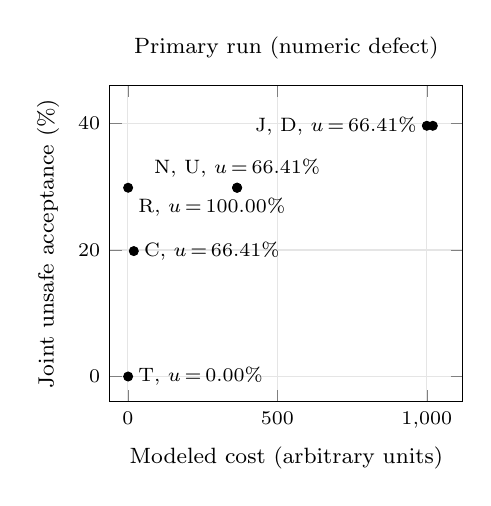
\begin{tikzpicture}[lbl/.style={font=\scriptsize, inner sep=3.5pt}]
\begin{axis}[width=0.5\textwidth, height=5.6cm, xmin=-60, xmax=1120, ymin=-4, ymax=46,
  title={Primary run (numeric defect)}, title style={font=\footnotesize},
  xlabel={Modeled cost (arbitrary units)}, ylabel={Joint unsafe acceptance (\%)},
  tick label style={font=\scriptsize}, label style={font=\footnotesize},
  grid=major, grid style={black!10}, clip=false]
\addplot[only marks, mark=*, mark size=1.6pt] coordinates {
  (\resPrimaryRulesOnlyCost,\resPrimaryRulesOnlyRisk)
  (\resPrimaryClassifierOnlyCost,\resPrimaryClassifierOnlyRisk)
  (\resPrimaryJudgeOnlyScriptedCost,\resPrimaryJudgeOnlyScriptedRisk)
  (\resPrimaryNaiveDelegationCost,\resPrimaryNaiveDelegationRisk)
  (\resPrimaryNaiveWithSinkCost,\resPrimaryNaiveWithSinkRisk)
  (\resPrimaryCheckedUncalibratedCost,\resPrimaryCheckedUncalibratedRisk)
  (\resPrimaryCheckedQuarantineCost,\resPrimaryCheckedQuarantineRisk)};
\node[lbl, anchor=north west] at (axis cs:\resPrimaryRulesOnlyCost,\resPrimaryRulesOnlyRisk)
  {R, $u$\,=\,\resPrimaryRulesOnlyUtility\%};
\node[lbl, anchor=west] at (axis cs:\resPrimaryClassifierOnlyCost,\resPrimaryClassifierOnlyRisk)
  {C, $u$\,=\,\resPrimaryClassifierOnlyUtility\%};
\node[lbl, anchor=south] at (axis cs:\resPrimaryNaiveWithSinkCost,\resPrimaryNaiveWithSinkRisk)
  {N, U, $u$\,=\,\resPrimaryNaiveWithSinkUtility\%};
\node[lbl, anchor=east] at (axis cs:\resPrimaryJudgeOnlyScriptedCost,\resPrimaryJudgeOnlyScriptedRisk)
  {J, D, $u$\,=\,\resPrimaryJudgeOnlyScriptedUtility\%};
\node[lbl, anchor=west] at (axis cs:\resPrimaryCheckedQuarantineCost,\resPrimaryCheckedQuarantineRisk)
  {T, $u$\,=\,\resPrimaryCheckedQuarantineUtility\%};
\end{axis}
\end{tikzpicture}\hfill
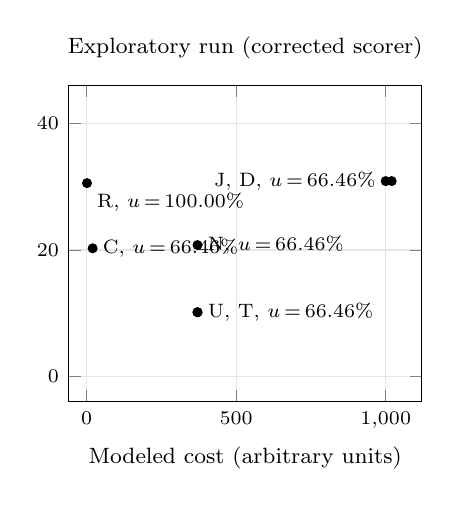
\begin{tikzpicture}[lbl/.style={font=\scriptsize, inner sep=3.5pt}]
\begin{axis}[width=0.5\textwidth, height=5.6cm, xmin=-60, xmax=1120, ymin=-4, ymax=46,
  title={Exploratory run (corrected scorer)}, title style={font=\footnotesize},
  xlabel={Modeled cost (arbitrary units)},
  tick label style={font=\scriptsize}, label style={font=\footnotesize},
  grid=major, grid style={black!10}, clip=false]
\addplot[only marks, mark=*, mark size=1.6pt] coordinates {
  (\resExploratoryRulesOnlyCost,\resExploratoryRulesOnlyRisk)
  (\resExploratoryClassifierOnlyCost,\resExploratoryClassifierOnlyRisk)
  (\resExploratoryJudgeOnlyScriptedCost,\resExploratoryJudgeOnlyScriptedRisk)
  (\resExploratoryNaiveDelegationCost,\resExploratoryNaiveDelegationRisk)
  (\resExploratoryNaiveWithSinkCost,\resExploratoryNaiveWithSinkRisk)
  (\resExploratoryCheckedUncalibratedCost,\resExploratoryCheckedUncalibratedRisk)
  (\resExploratoryCheckedQuarantineCost,\resExploratoryCheckedQuarantineRisk)};
\node[lbl, anchor=north west] at (axis cs:\resExploratoryRulesOnlyCost,\resExploratoryRulesOnlyRisk)
  {R, $u$\,=\,\resExploratoryRulesOnlyUtility\%};
\node[lbl, anchor=west] at (axis cs:\resExploratoryClassifierOnlyCost,\resExploratoryClassifierOnlyRisk)
  {C, $u$\,=\,\resExploratoryClassifierOnlyUtility\%};
\node[lbl, anchor=west] at (axis cs:\resExploratoryNaiveWithSinkCost,\resExploratoryNaiveWithSinkRisk)
  {N, $u$\,=\,\resExploratoryNaiveWithSinkUtility\%};
\node[lbl, anchor=west] at (axis cs:\resExploratoryCheckedQuarantineCost,\resExploratoryCheckedQuarantineRisk)
  {U, T, $u$\,=\,\resExploratoryCheckedQuarantineUtility\%};
\node[lbl, anchor=east] at (axis cs:\resExploratoryJudgeOnlyScriptedCost,\resExploratoryJudgeOnlyScriptedRisk)
  {J, D, $u$\,=\,\resExploratoryJudgeOnlyScriptedUtility\%};
\end{axis}
\end{tikzpicture}
\caption{Observed risk against modeled cost, with the primary and exploratory
runs shown separately. R: rules only; C: lexical only; J: scripted raw judge
only; D: invalid delegation; N: naive with sink; U: checked uncalibrated; T:
TINT (checked calibrated). Each label gives the benign utility $u$, which must
be read alongside the axes: the primary low-risk point denies all benign tasks.
Coincident or adjacent points share a label. These are local configurations, not Pareto frontiers of
real guard systems.}
\label{fig:tradeoffs}
\end{figure*}

Fig.~\ref{fig:tradeoffs} places the methods on risk and modeled cost. Rules
only remains far cheaper and has higher utility than TINT; TINT is not
dominant on every axis. Measured CPU time tells a similar story: TINT's
$p_{95}$ decision time is roughly twenty times that of the uncalibrated checked
core, and a separate microbenchmark attributes most of the gap to recomputing
the configuration fingerprint on every decision. Caching it per configuration
would remove the cost, at the price of a weaker binding between certificate and
running code. None of these timings estimates real guard inference latency.

\textbf{Distribution shift.} The shifted set contains only unauthorized patches
whose maintenance text is encoded, so it matches no listed string. The
structured view therefore shows a low score, no secret external payload and no
destructive production action, and TINT accepts
\resExploratoryShiftRisk{}\% of these attacks. The fingerprint still matches,
because a fingerprint identifies the configuration, not the input distribution.
In the primary run the same set was denied only because TINT denied
everything.

\textbf{Answer to RQ III.} On our authored mixture, TINT does not achieve a
better risk--utility--cost frontier than the simplest competent control in the
primary run, and in the corrected replication its advantage over
naive-with-sink comes entirely from denying judge-targeting text through the
structured view. Certification licensed a policy but improved no detection;
it neither recognized the implicit and encoded attacks nor noticed the shift.
We could not test real language models, state-of-the-art guards, realistic
tasks or adaptive attackers, so whether the formal assumptions hold in practice
remains open.

\subsection{Threats to validity}
\textbf{Internal validity.} The primary arithmetic defect is preserved, and the
correction is reported only as exploratory, on fresh seeds. We authored the
labels, templates and planted mutations, so they are not independent
observations of semantic safety. Regression tests check configuration identity,
not the correctness of arbitrary plugins. The original synthesis counts are
unavailable.

\textbf{External validity.} We evaluated no real base model, pretrained guard,
official defense implementation, external benchmark, completed development
task or practitioner workflow. Inference load, real token and GPU cost, long
sessions and temporal drift are untested. Local CPU times and modeled units
cannot establish deployment performance or savings.

\textbf{Construct validity.} The four denominators of
Definition~\ref{def:metrics} must not be interchanged. Benign acceptance is a
proxy, not task completion, and quarantine is not semantic noninterference.
A matching context identifier does not establish stationarity, and complete
dependency tracking remains a premise of the host.

\textbf{Conclusion validity.} Seeds resample one authored law, not independent
developers or tasks, and the agent-trace results are determined by family
masses. Conservative multiplicity correction can by itself produce
infeasibility. Our numeric lint traces every empirical number in the source to
a raw-derived summary but cannot inspect every glyph of the PDF.

\section{Related Work}
\label{sec:related}
\subsection{Guardrail systems}
Llama Guard, WildGuard, Constitutional Classifiers and ThinkGuard are
classification and reasoning approaches to safety
monitoring~\cite{arxiv231206674,arxiv240618495,arxiv250118837,arxiv250213458}.
NeMo Guardrails provides programmable rails, and LlamaFirewall combines
specialized scanners against agent threats~\cite{arxiv231010501,arxiv250503574};
OneShield illustrates configurable guardrail engineering~\cite{arxiv250721170}.
Truncated polynomial classifiers support progressive activation
monitoring~\cite{arxiv250926238}. These systems supply the heterogeneous layers
that a hierarchy composes, but they do not state the conditions under which one
layer's verdict may be reused by another. Our toy components do not reproduce
their learned behavior.

\subsection{Cascades and adaptive compute}
FrugalGPT studies cost-aware model cascades~\cite{arxiv230505176}. Trust or
Escalate provides cascaded selective evaluation with human-agreement
guarantees~\cite{arxiv240718370}, and Conformal Arbitrage calibrates a switch
between a primary model and a guardian and analyzes the optimality of
score-gap routing~\cite{arxiv250600911}. Hybrid abstention applies hierarchical
detection to practical filtering~\cite{arxiv260215391}. These works already
give calibrated cascades; we add a check that a certificate applies to the
actual route and input view at the tool-action boundary.
Proposition~\ref{thm:optimization} is a standard Lagrangian observation, not a
new routing theorem.

\subsection{Dual-process architectures}
The System~I/System~II vocabulary links fast response with deliberate
reasoning, and a recent survey organizes the reasoning-model
literature~\cite{arxiv250217419}. We use only an operational resource
criterion. Training for helpfulness and harmlessness and constitutional
feedback address safety at training time~\cite{arxiv220405862,arxiv221208073};
they complement but do not replace mediation of tool effects.

\subsection{Runtime enforcement and verification}
AgentSpec provides a rule language for runtime constraints on
agents~\cite{arxiv250318666}; ShieldAgent reasons over verifiable policy
representations~\cite{arxiv250322738}; ProbGuard monitors predicted future
safety probabilistically~\cite{arxiv250800500}; and VeriGuard separates offline
verification of a policy from online monitoring of actions~\cite{arxiv251005156}.
ContrAgent is the closest work, with temporal agent contracts and compiled
monitors~\cite{arxiv260918128}, and Agent Behavioral Contracts add composition
and probabilistic satisfaction~\cite{arxiv260222302}. The layered
probabilistic architecture of~\cite{arxiv260518672} already composes
conditional safety guarantees, which rules out any claim that ours is the
first such composition. Classical shield synthesis corrects actions at run time
against formal specifications~\cite{arxiv150102573,arxiv170808611,arxiv190805402,arxiv240604184},
and RoboGuard protects a root-of-trust model with temporal
constraints~\cite{arxiv250307885}. TINT's deterministic mediation belongs to
this lineage; what it adds is an executable check of delegation premises
between heterogeneous layers.

\subsection{System-level isolation}
CaMeL separates control flow from data flow and mediates
capabilities~\cite{arxiv250318813}, and Fides tracks confidentiality and
integrity labels with a formal planner model~\cite{arxiv250523643}. These
systems give stronger isolation than our structured judge view. Spotlighting
and instruction-hierarchy training instead rely on model behavior to respect
provenance cues and instruction priority~\cite{arxiv240314720,arxiv240413208}.
Our quarantine is a deliberately narrow input schema, not evidence that prompt
formatting prevents instruction following. Task Shield checks alignment with
the user's goal and would be a stronger real-agent comparison
target~\cite{arxiv241216682}.

\subsection{Statistical guarantees}
CRC controls expected monotone loss under exchangeability~\cite{arxiv220802814}.
Conformal tutorials and adaptive classification methods distinguish marginal
from conditional guarantees~\cite{arxiv210707511,arxiv200602544}. Adaptive
conformal inference addresses changing distributions, and later methods
broaden the controlled objectives to adaptive and tail
risks~\cite{arxiv210600170,arxiv240617819,arxiv250220285}. Conformal
abstention, factuality and language-generation methods provide further
statistical interfaces~\cite{arxiv240501563,arxiv240210978,arxiv230610193}. We
use a classical finite-family binomial certificate and claim no new conformal
result or adaptive guarantee.

\subsection{Layered safety engineering}
Component contracts, runtime assurance and defense in depth all argue for
exposing assumptions rather than counting layers. ScenicProver is a closely
related compositional assurance framework that tracks evidence and
provenance~\cite{arxiv251102164}. Semantic integrity constraints show
declarative assurance at another software boundary~\cite{arxiv250300600}, and
NaSh emphasizes recovery and guardrail design for language-driven
shells~\cite{arxiv250613028}. Our contribution is an executable integration
for a restricted tool-agent interface, not a new safety-case principle.

\subsection{Attacks and evaluation}
Indirect prompt injection, optimized jailbreaks, guard evasion and attacks on
latent defenses show that guard behavior must itself be part of the threat
model~\cite{arxiv230212173,arxiv230715043,arxiv250411168,arxiv241209565,arxiv250305264}.
Retrieved context can change guard judgments~\cite{arxiv251005310}, and
baseline defenses show why attacker access must be
specified~\cite{arxiv230900614}. AgentDojo, ASB, AgentHarm, RedCode, ToolEmu and
R-Judge offer much richer evaluation
substrates~\cite{arxiv240613352,arxiv241002644,arxiv241009024,arxiv241107781,arxiv230915817,arxiv240110019},
and RedCodeAgent, BAD-ACTS and CyberSecEval extend agent-security
testing~\cite{arxiv251002609,arxiv250816481,arxiv240801605}. Sensitivity to
representation cautions against reading a benchmark score as an intrinsic model
property~\cite{arxiv261003585}. We executed none of these benchmarks, and our
fixture search is not comparable to them.

\begin{table*}[t]
\caption{Comparison with the closest work. Y: capability established in the
reviewed source; S: a different or narrower property; U: not established in
our review (never a claim of absence); P: proposed and tested only in our
local pilot.}
\label{tab:gap}
\centering\scriptsize
\begin{tabular}{lccccccccc}
\toprule
Approach & Hierarchy & Formal spec & Hard & Statistical & Conditioned trust & Cost & Agent traces & Adaptive & Tool\\
\midrule
ContrAgent & U & Y & Y & U & Y & Y & Y & U & Y\\
Layered probabilistic contracts & Y & Y & S & Y & Y & U & U & U & U\\
Conformal Arbitrage & Y & Y & U & Y & S & Y & U & U & Y\\
Trust or Escalate & Y & Y & U & Y & S & Y & U & U & Y\\
AgentSpec & U & Y & Y & U & U & Y & Y & U & Y\\
CaMeL / Fides & Y & Y & Y & U & Y & Y & Y & Y & Y\\
RoboGuard & Y & Y & Y & U & Y & Y & Y & Y & Y\\
ScenicProver & Y & Y & Y & Y & Y & S & S & U & Y\\
TINT local integration & Y & Y & P & P & Y & P & P & U & Y\\
\bottomrule
\end{tabular}
\end{table*}

In Table~\ref{tab:gap}, \emph{hierarchy} means composed guards; \emph{formal
spec}, machine-defined constraints; \emph{hard}, exact safety within a stated
semantics; \emph{statistical}, a probability guarantee; \emph{conditioned
trust}, explicit reliance premises; \emph{cost}, resource-aware routing or
measurement; \emph{agent traces}, tool-action sequences; \emph{adaptive},
analyzed response-informed attacks; and \emph{tool}, an available artifact.
TINT's adaptive cell is U because our fixture search is not such an analysis.
No single column is claimed as novel; the table shows that TINT's
combination is unusual, not that any part of it is new.

\section{Discussion and Limitations}
\label{sec:discussion}
\textbf{Lessons.} Four lessons generalize beyond our toy instrument.
\emph{First, make premises executable.} The counterexample of
Proposition~\ref{thm:nontransitive} is trivial on paper, yet the naive
hierarchy it describes is easy to build. Checking the judge's input view on
every call turned an implicit assumption into a denial. \emph{Second, keep the
mandatory checks at the sink.} In our data the sink alone stopped every hard
violation, including canonical $T_j$; conditioned trust adds value only for
semantic attacks the sink cannot decide. \emph{Third, certification licenses
but does not detect.} The certificate decided whether a policy could run; it
could not make a detector see implicit or encoded attacks, and a matching
fingerprint did not reveal the shift. Teams that calibrate a guard should
expect to learn that it is inadequate, as we did, and should design the
system so that this outcome is reported rather than hidden. \emph{Fourth,
inspect the policy grid before calibrating.} A grid whose thresholds all give
the same risk cannot be rescued by any statistical procedure; a check of how
many behaviorally distinct policies a grid contains would have revealed the
primary infeasibility before the run.

\textbf{Limitations.} The canonical counterexample also shows that ordinary
mediation already protects the hard property, and the route sums only prevent
a known error: importing ensemble intersections into early-exit accounting.
These are established principles made executable, not new safety laws. All
empirical evidence comes from an authored mixture with scripted guards whose
decisions are fixed by family, so the study demonstrates mechanisms, not
effectiveness. The distinctive practical value of conditioned trust therefore
remains a research question.

\textbf{What a convincing evaluation needs.} A follow-up study should use real
proposal-generating models and independently implemented learned guards on
external benchmarks such as AgentDojo, compare against the official
implementations of the closest systems, and measure task completion rather
than benign acceptance. GPU-hosted models, activation probes and reasoning
judges may change miss rates, correlations, costs and latency under load; no
number reported here should be expected to transfer. Further work also needs
richer rule semantics, separately calibrated route bounds, independently
authored policy errors, adaptive attacks that observe guard responses, and a
proved refinement link between the abstraction and the implementation.

\section{Conclusion}
Trust between guard layers is conditional, and conditions that are not checked
are not guarantees. TINT makes a limited assurance case executable:
deterministic effects stay mediated, certificates are bound to the actual
routing configuration, and unproved premises are visible. Scoped proofs and
reproducible experiments separate conditional component guarantees from valid
composition. The empirical picture is sobering: the primary certified runtime
was safe only by refusing all work, the corrected replication still accepted
implicit attacks, and the shifted attacks passed unnoticed. Establishing
real-agent engineering value is the next step.

\section*{Data and Artifact Availability}
The repository is \url{https://github.com/ai4se4ai-lab/trust-is-not-transitive}.
It contains compressed raw decision logs, processed summaries, hashes of
sources and configurations, proofs (Propositions~\ref{thm:nontransitive}--\ref{thm:limits}
correspond to \texttt{T0}--\texttt{T4} in \texttt{formal/FRAMEWORK.md}), the
PRISM input and output, generated macros and vector figures. The commit that
produced each raw run is recorded in its \texttt{environment.json}, and the
artifact manifest identifies the analysis inputs. Both the historical primary
scorer and the corrected exploratory scorer are retained. \texttt{ARTIFACT.md}
distinguishes re-analysis from full reruns and lists unavailable
prerequisites. No archival release or DOI has been created yet.

\section*{Ethics and Acknowledgments}
All attack strings target the local typed interpreter or a scripted judge.
The released fixtures involve no real network egress, production operation,
third-party exploit, personal data or genuine secret. No study with human
participants was conducted. We did not accept access conditions for external
models, and we do not redistribute external datasets. No funding or
institutional approval is claimed. Automated reviews used during development
are aids to the authors, not independent peer review.

\bibliographystyle{IEEEtran}
\bibliography{references}
\end{document}
